%%%%%%%%%%%%%%%%%%%%%%%%%%%%%%%%%%%%%%%%%%%%%%%%%%%%%%%
%
%                             
%
% \documentclass{woosterthesis} must be at the beginning of every IS. Options are the same as
% for the report class with some additional options: abstractonly, acs, alltt, apa, blacklinks, chicago,
% code, colophon, dropcaps, euler, foreignlanguage, gauss, index, kaukecopyright, lshortwooster, maple, mla, palatino, picins,tikz,
% verbatim, wblack, and woostercopyright. The kaukecopyright option will put the arch symbol with the word mark on the
% copyright page. The woosterthesis class is based on the report class. One thing to note is that
% the ``%'' symbol comments out all characters that follow it on the line.
%
%%%%%%%%%%%%%%%%%%%%%%%%%%%%%%%%%%%%%%%%%%%%%%%%%%%%%%%

%%%%%%%%%%%%%%%%%%%%%%%%%%%%%%%%%%%%%%%%%%%%%%%%%%%%%%%
%
% Checked on 8/26/22 and compiles with no fatal errors. Users must have the latest version of the TeXLive software and
% have installed all available packages from CTAN to ensure this thesis class compiles with no fatal errors. Also, you must
% run pdfLaTex, Biber, MakeIndex, padfLaTeX, pdfLaTeX to get all the numbering and references resolved. This is the
% first year the template uses Biber for references.
%
%%%%%%%%%%%%%%%%%%%%%%%%%%%%%%%%%%%%%%%%%%%%%%%%%%%%%%%

%%%%%%%%%%%%%%%%%%%%%%%%%%%%%%%%%%%%%%%%%%%%%%%%%%%%%%%
% use this declaration for a draft  version of your IS
\documentclass[palatino,code,picins,tikz,kaukecopyright,openright,lshortwooster,dropcaps,verbatim,index,oneside,euler,final]{woosterthesis}
% Note that you can specify the acs option to use the American Chemical Society citation format, apa option to use the American
% Psychological Association citation format, chicago option to use the Chicago citation format, mla option to use the Modern Language
% Association citation format, wblack option for a grayscale Wooster "W" on the cover, and scottie option for a grayscale Scottie Mascot
% on the cover. See exampleis_manual.pdf for an explanation of all the options.
%
%%%%%%%%%%%%%%%%%%%%%%%%%%%%%%%%%%%%%%%%%%%%%%%%%%%%%%%
%
% use this declaration for the print version of your IS
%\documentclass[12pt,code,palatino,picins,blacklinks,kaukecopyright,openright,oneside,final]{woosterthesis} % probably what most students would use
%
%%%%%%%%%%%%%%%%%%%%%%%%%%%%%%%%%%%%%%%%%%%%%%%%%%%%%%%
%

% use this declaration for the PDF version of your IS
%\documentclass[12pt,code,palatino,picins,kaukecopyright,openright,oneside,final]{woosterthesis}
%
%%%%%%%%%%%%%%%%%%%%%%%%%%%%%%%%%%%%%%%%%%%%%%%%%%%%%%%

%%%%%%%%%%%%%%%%%%%%%%%%%%%%%%%%%%%%%%%%%%%%%%%%%%%%%%%
%
%                                                       Load Packages
%
%   To load packages in addition to the ones that are loaded by default, please place your
%   usepackage commands in the packages.tex file in the styles folder.
%
%%%%%%%%%%%%%%%%%%%%%%%%%%%%%%%%%%%%%%%%%%%%%%%%%%%%%%%

%%%%%%%%%%%%%%%%%%%%%%%%%%%%%%%%%%%%%%%%%%%%%%%%%%%%%%%%%%%%%%%%%%%%%%%%%%%%%%%%%%%%%%%%%%%%%%
%
%                                                       Packages
%
% Do not add any other packages without consulting with Dr. Breitenbucher as they may break the functionality of the class.
%
%%%%%%%%%%%%%%%%%%%%%%%%%%%%%%%%%%%%%%%%%%%%%%%%%%%%%%%%%%%%%%%%%%%%%%%%%%%%%%%%%%%%%%%%%%%%%%

% --- Font definitions if you are using XeLaTeX engine instead of PDFLaTeX engine ---
\ifxetex%
	\defaultfontfeatures{Ligatures=TeX,Mapping=tex-text,Renderer=ICU} %
		\setmainfont[Numbers=OldStyle]{Times New Roman} % default Times New Roman, other choices for the main font would be Libertinus Serif, TeX Gyre Pagella. XITS, STIX Two Text, Fira Sans Book, Cambria, Latin Modern Roman
		\setmathfont{TeX Gyre Termes Math} % default TeX Gyre Termes Math, other choices for the math font would be Libertinus Math, TeX Gyre Pagella Math, XITS Math, STIX Two Math, Fira Math, Cambria Math (Windows), Latin Modern Math
		\setsansfont[Scale=.87,Fractions=On,Numbers=Lining]{Arial}% default Arial, other choices for the sans serif font would be Skia, Arial, Helvetica, Helvetica Neue, Libertinus Sans, TeX Gyre Heros, Source Sans Pro, Fira Sans, Calibri, Latin Modern Sans
		\setmonofont[Scale=.9]{Courier New} % default Courier New, other choices for the mono font would be Libertinus Mono, TeX Gyre Cursor, Source Code Pro, Fira Mono, Consolas, Latin Modern Mono
\fi

%%%%%%%%%%%%%%%%%%%%%%%%%%%%%%%%%%%%%%%%%%%%%%%%%%%%%%%
%
%                                                       Load Personal commands
%                                                                    
%  There will be certain commands that you use frequently in the thesis. You can give these
%  commands new names which are easier for you to remember. You can also combine several
%  commands into a new command of your own. See The LaTeX Companion or Guide to LaTeX
%  for examples on defining your own commands. These are commands that I defined to cut
%  down on typing. You can enter your commands in the personal.tex file in the styles folder.
%
%%%%%%%%%%%%%%%%%%%%%%%%%%%%%%%%%%%%%%%%%%%%%%%%%%%%%%%

%%%%%%%%%%%%%%%%%%%%%%%%%%%%%%%%%%%%%%%%%%%%%%%%%%%%%%%%%%%%%%%%%%%%%%%%%%%%%%%%%%%%%%%%%%%%%%
%
%                                                       Personal Commands
%                                                                    
% There will be certain commands that you use frequently in the thesis. You can give these
% commands new names which are easier for you to remember. You can also combine several
% commands into a new command of your own. See The LaTeX Companion or Guide to LaTeX for
% examples on defining your own commands. These are commands that I defined to cut down on typing.
%
%%%%%%%%%%%%%%%%%%%%%%%%%%%%%%%%%%%%%%%%%%%%%%%%%%%%%%%%%%%%%%%%%%%%%%%%%%%%%%%%%%%%%%%%%%%%%%

\newcommand{\fl}{\ell}
\newcommand{\lt}{\LaTeX\ }
\newcommand{\msw}{Word\texttrademark\ }
\newcommand{\xt}{\ifthenelse{\boolean{xetex}}{\XeTeX\ }{XeTeX} }
%\newcommand{\Cl}{\ensuremath{\textup{C}_\fl}}
%\newcommand{\bCl}{C$_{\ell}$}
%\newcommand{\Al}{\ensuremath{\textup{A}_\fl}}
%\newcommand{\msum}{{(m_1+\cdots+m_\ell)}}
%\newcommand{\Nsum}{{(N_1+\cdots+N_\ell)}}
%\newcommand{\ysum}{{(y_1+\cdots+y_\ell)}}
%\newcommand{\Nsub}{{N_1+\cdots+N_\ell}}
%\newcommand{\ysub}{{y_1+\cdots+y_\ell}}
%\newcommand{\xsub}{{x_1+\cdots+x_\ell}}
%\newcommand{\ysqsum}{{y_1^2+\cdots +y_{\fl}^2}}
%\newcommand{\msqsum}{{m_1^2+\cdots +m_{\fl}^2}}
%\newcommand{\ratio}{\left(\frac{\beta}{\alpha}\right)}
%\newcommand{\LT}{\ensuremath{\LaTeX{}}}

%%%%%%%%%%%%%%%%%%%%%%%%%%%%%%%%%%%%%%%%%%%%%%%%%%%%%%%%%%%%%%%%%%%%%%%%%%%%%%%%%%%%%%%%%%%%%%
% These commands have one argument and are entered as \commandname{argument}.
%%%%%%%%%%%%%%%%%%%%%%%%%%%%%%%%%%%%%%%%%%%%%%%%%%%%%%%%%%%%%%%%%%%%%%%%%%%%%%%%%%%%%%%%%%%%%%

%\newcommand{\bd}[1]{\textbf{#1}}
\newcommand{\mbd}[1]{{\mathbf{#1}}}
%\newcommand{\abs}[1]{\vert{#1}\vert}
\newcommand{\bvec}[1]{{\mbd{#1}}}
%\newcommand{\lvec}[1]{\abs{\bvec{#1}}}
%\newcommand{\nesmallprod}[1]{\prod_{\substack{#1=1\\
%#1\neq p}}^{\fl}}
%\newcommand{\esec}[1]{e_{2}({#1}_1,\ldots ,{#1}_\fl)}
%\newcommand{\smallprod}[1]{\prod_{#1=1}^{\fl}}
%\newcommand{\incsum}[1]{{#1}_2+2{#1}_3+\cdots +(\fl -1){#1}_\fl}
%\newcommand{\binomsum}[1]{\binom{{#1}_1}{2}+\cdots +\binom{{#1}_\fl}{2}}
%\newcommand{\imultsum}[1]{\multsum{{#1}_k\ge 0}{k=1,\ldots ,\fl}}
%\newcommand{\diagsum}[1]{\sum _{\substack{{#1}_k\ge 0\\
%k=1, \ldots ,\fl\\
%\lvec{#1}=m}}}
%\newcommand{\Mb}[1][\fl]{\ensuremath{\textup{\bd{M}}_b^{(#1)}}}
%\newcommand{\HLV}[1]{\ensuremath{\textup{\bd{H}}_{#1}}}
%\newcommand{\Rq}[1][p]{\ensuremath{\textup{R}_q^{(#1)}}}
\newcommand{\degree}[1]{\ensuremath{#1^{\circ}}}
\newcommand{\ip}[1]{\texttt{#1}\index{packages!#1}}
\newcommand{\ic}[1]{\texttt{$\backslash$#1}\index{commands!#1}}
\newcommand{\ie}[1]{#1\index{#1}}

%%%%%%%%%%%%%%%%%%%%%%%%%%%%%%%%%%%%%%%%%%%%%%%%%%%%%%%%%%%%%%%%%%%%%%%%%%%%%%%%%%%%%%%%%%%%%%
% These commands have 2 or more arguments some with default values for the first argument. You
% can learn a lot about constructing complicated equations by studying the commands in this %section.
%%%%%%%%%%%%%%%%%%%%%%%%%%%%%%%%%%%%%%%%%%%%%%%%%%%%%%%%%%%%%%%%%%%%%%%%%%%%%%%%%%%%%%%%%%%%%%

%\newcommand{\qbinom}[2]{\ensuremath{\left[{#1}\atop{#2}\right]_q}}
%\newcommand{\sqprod}[2]{\prod_{#1,#2=1}^{\fl}}
%\newcommand{\triprod}[2]{\prod_{1\le #1<#2\le \fl}}
%\newcommand{\nesqprod}[2]{\prod_{\substack{#1,#2=1\\
%#1,#2\neq p}}^{\fl}}
%\newcommand{\netriprod}[2]{\prod_{\substack{1\le #1<#2\le \fl\\
%#1,#2\neq p}}}
\newcommand{\qrfac}[3][\ ]{\left({#2}\right)_{#3}^{#1}}
%\newcommand{\multsum}[2]{\sum_{\substack{{#1}\\
%\\
%{#2}}}}
%\newcommand{\fmultsum}[2][N]{\multsum{0\le {{#2}_k}\le {{#1}_k}}{k=1,\ldots ,\fl}}
%\newcommand{\pq}[2]{\ _{#1}\varphi_{#2}}
%\newcommand{\mess}[2][y_k]{\frac{\qrfac{\alpha x_k}{#2}\qrfac{qx_k\beta^{-1}}{#2}}{\qrfac{\beta x_k}{#1}
%\qrfac{qx_k\alpha^{-1}}{#1}}}
%\newcommand{\MG}[7][\fl]{\ensuremath{\left[\textup{MG}\right]_{#2}^{(#1)}{#3}q;{#4};{#5}^{#6}{#7}}}

%%%%%%%%%%%%%%%%%%%%%%%%%%%%%%%%%%%%%%%%%%%%%%%%%%%%%%%%%%%%%%%%%%%%%%%%%%%%%%%%%%%%%%%%%%%%%%
% These commands define new environments
%%%%%%%%%%%%%%%%%%%%%%%%%%%%%%%%%%%%%%%%%%%%%%%%%%%%%%%%%%%%%%%%%%%%%%%%%%%%%%%%%%%%%%%%%%%%%%

\newcounter{unnumft}
\setcounter{unnumft}{0}
\newenvironment{unnumft}[2]{\renewcommand{\thefootnote}{}\footnote{#1}\footnote{#2}} {\addtocounter{footnote}{-2}}
\newenvironment{wooexample}{\small
\begin{singlespace}
\begin{example}}{\end{example}
\end{singlespace}}

\graphicspath{{./figures/}}% for setting where to look for figures
%\citestyle{wooster}% change the style of citations. Math and CS people should leave this alone.

%%%%%%%%%%%%%%%%%%%%%%%%%%%%%%%%%%%%%%%%%%%%%%%%%%%%%%%%%%%%%%%%%%%%%%%%%%%%%%%%%%%%%%
% Modify the formatting of the back references
%%%%%%%%%%%%%%%%%%%%%%%%%%%%%%%%%%%%%%%%%%%%%%%%%%%%%%%%%%%%%%%%%%%%%%%%%%%%%%%%%%%%%%
\DefineBibliographyStrings{english}{%
	backrefpage  = {page }, % for single page number
	backrefpages = {pages } % for multiple page numbers
}






%%%%%%%%%%%%%%%%%%%%%%%%%%%%%%%%%%%%%%%%%%%%%%%%%%%%%%%
%
%                                                       Load Theorem formatting information
%
%  If you need to define an new theorem style or want to see what theorem like environments 
%  are available please look at the theorems.tex file in the styles folder.
%
%%%%%%%%%%%%%%%%%%%%%%%%%%%%%%%%%%%%%%%%%%%%%%%%%%%%%%%

%%%%%%%%%%%%%%%%%%%%%%%%%%%%%%%%%%%%%%%%%%%%%%%%%%%%%%%%%%%%%%%%%%%%%%%%%%%%%%%%%%%%%%%%%%%%%%
%
% This is where one would tell \LaTeX{} how to format Theorems, Definitions, etc. and also
% indicate the environment names. You need the amsthm package (loaded in the woosterthesis %class) in order for these commands to work.
%
%%%%%%%%%%%%%%%%%%%%%%%%%%%%%%%%%%%%%%%%%%%%%%%%%%%%%%%%%%%%%%%%%%%%%%%%%%%%%%%%%%%%%%%%%%%%%%

% an example of defining your own theoremstyle
%\newtheoremstyle{break}% name
%  {\topsep}%      Space above
%  {\topsep}%      Space below
%  {\itshape}%         Body font
%  {}%         Indent amount (empty = no indent, \parindent = para indent)
%  {\bfseries}% Thm head font
%  {.}%        Punctuation after thm head
%  {\newline}%     Space after thm head: " " = normal interword space;
%        %       \newline = linebreak
%  {}%         Thm head spec (can be left empty, meaning `normal')
% Kyle Kindbom requested a theorem style where the theorem header was on a separate line.
% The break theorem style will put a line break after the theorem header. - JB
\newtheoremstyle{break}% name
	{\topsep}%	Space above
	{\topsep}%	Space below
	{\itshape}%	Body font
	{}%			Indent amount (empty = no indent, \parindent = para indent)
	{\bfseries}%	Thm head font
	{.}%			Punctuation after thm head
	{\newline}%	Space after thm head: " " = normal interword space;
	%		\newline = linebreak
	{}%			Thm head spec (can be left empty, meaning `normal')
\newtheoremstyle{scthm}{\topsep}{\topsep}{\itshape}{}{\bfseries\scshape}{}{ }{}% small cap font for the heading
\newtheoremstyle{itdefn}{\topsep}{\topsep}{\itshape}{}{\bfseries}{.}{ }{}% italic definitions
\newtheoremstyle{scdefn}{\topsep}{\topsep}{\itshape}{}{}{}{ }{\thmname{\textbf{#1}}\thmnumber{ \textbf{#2}}\thmnote{ \scshape #3:}}% small cap headings and italic text.

\theoremstyle{break}% this theoremstyle will put the text of the theorem on a new line.
\newtheorem{thm}{Theorem}[chapter]%number theorems within chapters 
%\newtheorem{cor}[thm]{Corollary}%by using [thm] we are numbering these environments with the theorems.
\newtheorem{cor}{Corollary}[chapter]%number corollaries within chapters .
%\newtheorem{lem}[thm]{Lemma}
\newtheorem{lem}{Lemma}[chapter]
%\newtheorem{prop}[thm]{Proposition}
\newtheorem{prop}{Proposition}[chapter]

\theoremstyle{scdefn}
%\newtheorem{defn}[thm]{Definition}
\newtheorem{defn}{Definition}[chapter]
\theoremstyle{remark}
%\newtheorem{rem}[thm]{Remark}
\newtheorem{rem}{Remark}[chapter]
\renewcommand{\therem}{}
%\newtheorem{ex}[thm]{Example}
\newtheorem{ex}{Example}[chapter]

\theoremstyle{plain}
%\newtheorem{note}[thm]{Notation}
\newtheorem{note}{Notation}[chapter]
\renewcommand{\thenote}{}
%\newtheorem{nts}[thm]{Note to self}%use to remind yourself of things yet to do
\newtheorem{nts}{Note to self}[chapter]
\renewcommand{\thents}{}
%\newtheorem{terminology}[thm]{Terminology}
\newtheorem{terminology}{Terminology}[chapter]
\renewcommand{\theterminology}{}

\theoremstyle{itdefn}
\newtheorem{bdefn}{Definition}[chapter]
\newsavebox{\fmbox} 
\newenvironment{boxeddefn}[2] 
{\begin{lrbox}{\fmbox}\begin{minipage}{0.9 \linewidth }\begin{singlespace}\begin{bdefn}[{#1}]\label{#2}\vspace{0.2cm}} 
{\end{bdefn}\end{singlespace}\end{minipage}\end{lrbox}\fbox{\usebox{\fmbox}}}

\setcounter{secnumdepth}{5}% controls the numbering of sections
\setcounter{tocdepth}{6}% controls the number of levels in the Contents

%%%%%%%%%%%%%%%%%%%%%%%%%%%%%%%%%%%%%%%%%%%%%%%%%%%%%%%
%
%  This is where one enters their bibilography file name.
%
%%%%%%%%%%%%%%%%%%%%%%%%%%%%%%%%%%%%%%%%%%%%%%%%%%%%%%%

\addbibresource{references.bib}

%%%%%%%%%%%%%%%%%%%%%%%%%%%%%%%%%%%%%%%%%%%%%%%%%%%%%%%
%
%  This is where one enters the information about the thesis.
%
%%%%%%%%%%%%%%%%%%%%%%%%%%%%%%%%%%%%%%%%%%%%%%%%%%%%%%%

\title{Computational Identification of High-Altitude Molecules Using Molecular Networking and Liquid Chromatography High-Resolution Mass Spectrometry (LC-HRMS): Developing Software by Chemists, for Chemists}
\thesistype{Independent Study Thesis} % you should make this Independent Study Thesis
\author{Raelyn Brooks} % you should put your name here
%\presentdegrees{Ph.D.} % you should comment this line
\degreetoobtain{Bachelor of Arts} % you should put your degree here
\presentschool{The College of Wooster}
\academicprogram{Departments of Chemistry \& Computer Science} % you should put your department here
\gradyear{2027}
\advisor{Jennifer Faust (Chemistry)}
\secondadvisor{John Musgrave (Computer Science)}
%\reader{Reader}
\copyrighted   
%\copyrightdate{}                  
\makeindex % comment this line if you do not have an index

%%%%%%%%%%%%%%%%%%%%%%%%%%%%%%%%%%%%%%%%%%%%%%%%%%%%%%%
%
%  This is where the commands for the document begin. All \LaTeX{} documents must have a
%  \begin{document} text .... \end{document} structure.
%
%%%%%%%%%%%%%%%%%%%%%%%%%%%%%%%%%%%%%%%%%%%%%%%%%%%%%%%

\begin{document}

%%%%%%%%%%%%%%%%%%%%%%%%%%%%%%%%%%%%%%%%%%%%%%%%%%%%%%%
%
%  The front matter includes acknowledgments, dedications, vitas, list of tables, list of figures,
%  copyright, abstract, title page, and contents.
%
%%%%%%%%%%%%%%%%%%%%%%%%%%%%%%%%%%%%%%%%%%%%%%%%%%%%%%%

\frontmatter
\ifthenelse{\boolean{abstractonly}}{
  % Do nothing — skip front matter
}{
\maketitle
\ClearShipoutPicture
\clearpage\thispagestyle{empty}\null\clearpage
\disscopyright 
}

%%%%%%%%%%%%%%%%%%%%%%%%%%%%%%%%%%%%%%%%%%%%%%%%%%%%%%%
%                                                                                       
%                                                       Abstract						
%                                                                                       
%%%%%%%%%%%%%%%%%%%%%%%%%%%%%%%%%%%%%%%%%%%%%%%%%%%%%%%

\begin{abstract}
Include a short summary of your thesis, including any pertinent results.  This section is \emph{not} optional, and the reader should be able to learn the meat of your thesis by reading this (short) section.
\end{abstract}

%%%%%%%%%%%%%%%%%%%%%%%%%%%%%%%%%%%%%%%%%%%%%%%%%%%%%%%
%                                                                                       
%                                                       Dedications					
%                                                                                       
%%%%%%%%%%%%%%%%%%%%%%%%%%%%%%%%%%%%%%%%%%%%%%%%%%%%%%%

\dedication{This work is dedicated to the future generations of Wooster students.}


%%%%%%%%%%%%%%%%%%%%%%%%%%%%%%%%%%%%%%%%%%%%%%%%%%%%%%%
%                                                                                       
%                                                       Acknowledgments					
%                                                                                       
%%%%%%%%%%%%%%%%%%%%%%%%%%%%%%%%%%%%%%%%%%%%%%%%%%%%%%%

\begin{acknowl}  
No part of my journey at The College of Wooster has been accomplished alone. Behind every class, project, difficult conversation, and moment of growth are people who have supported me, challenged me, and reminded me why I started. This Independent Study is no exception. I am grateful to everyone who helped me become not only a better student and researcher, but also a better person.

First, I want to thank my Senior Independent Study advisors, Dr.~Faust and Dr.~Musgrave, for guiding me through a project that brings chemistry and computer science together. Dr.~Faust, you have been one of my biggest champions. Thank you for believing in me, advocating for me, and helping me see what I am capable of even when I have struggled to see it myself. Dr.~Musgrave, thank you for your guidance, patience, and willingness to work through the challenges of turning an interdisciplinary idea into a meaningful computer science project. I am also grateful to Dr.~Paul Edmiston for bringing the original molecular-networking problem to my attention and giving me a reason to explore how the two disciplines I love could work together.

To the Computer Science Department, thank you for teaching me how to think critically, build things, and persist when the first solution fails. Dr.~Heather Guarnera, thank you for always helping me find a way to make the impossible seem possible. Dr.~Drew Guarnera, as my first computer science professor, you helped build a foundation that continues to shape my work. Dr.~Palmer, thank you for contributing to my growth as a programmer and computer scientist. I am grateful to the rest of the department as well, including the faculty and staff whose time, encouragement, and teaching helped me find my place in the field.

To the Chemistry Department, thank you for making science something I wanted not only to study, but to spend my life exploring. Dr.~Martin, thank you for your guidance as my academic advisor and for supporting my path across two majors. Dr.~Snider, thank you for the difficult but necessary conversation that helped me grow. Dr.~Bonvallet, thank you for making lectures something to look forward to. Dr.~Gallo, thank you for helping me fall in love with chemistry. Dr.~Baker, thank you for being one of my favorite professors and one of my favorite people to stop and say hello to. Dr.~Feierabend, thank you for pushing me to be great, especially in the moments when I did not fully believe I could be. I am grateful to every other member of the Chemistry Department who shared their knowledge, offered encouragement, or made the department feel like a community.

To my best friends, Kate Carson, Eliza Davis, and Brooke Bradley, thank you for being part of my life through the busy days, the stressful weeks, and the moments worth celebrating. Your friendship has meant more to me than I can put into a single paragraph. Thank you for giving me people I could laugh with, rely on, and be myself around.

To my brothers of Beta Kappa Phi, thank you for giving me a brotherhood and a home within Wooster. I especially want to recognize Shea McLaren, Cooper Norwell, Gabriel Jones, Nathan Krieg, Parth, Isaac Prince, Jackson Ferrell and Matthew Dalton, my littles, Hayden Jacoby and Peter Dentzer, my grand big and big. Each of you has helped shape what brotherhood, responsibility, and friendship mean to me. I am proud of the memories we have made and the people we have become together. The first and finest will always hold a special place in my heart.

To the Residence Life Office, thank you for the opportunity to grow as a leader and learn what it means to show up for a community. I also want to thank Maddie Cuckow, my former AD and now Greek Life Director, for being part of that journey and for the support and guidance you have given me along the way.

I want to give a special thank-you to Lauren Richmond, who has been an important part of my life and personal growth throughout the years. Although life has taken us in different directions, I will always be grateful for the love, encouragement, and support she has given me. The memories we created, the challenges we faced, and the experiences we shared have shaped me in ways I will always appreciate. Her impact on my journey extends far beyond our time together, and I will always value the role she played in helping me become the person I am today.

To Ty Reynolds, Doug Slovenkay, Ethan Hunt, Taryn Brady, Saveer Patil, Levi Monroe, Ben Kimble, Madeline Eaton, and Sofia Wolken, thank you for being part of my college experience. Whether through conversation, friendship, encouragement, or simply being present along the way, you have each contributed to memories and experiences I will carry with me beyond Wooster.

To Fr.~David, thank you for walking alongside me during my journey toward baptism. Your guidance helped me through a deeply personal part of my life, and I am grateful for the time, care, and faith you shared with me.

Most importantly, I thank my family and siblings, especially my seven sisters and six brothers. You are part of the reason I care so deeply about using what I learn to make a difference. Thank you for the love, sacrifices, patience, and encouragement that have carried me through every stage of my education. Whatever I accomplish, I will always carry my family with me.

Finally, to everyone whose name may not appear here but who has offered a kind word, a difficult lesson, a new opportunity, or a reason to keep going, thank you. This work may have my name on its cover, but the person who completed it was shaped by all of you.
\end{acknowl}

%%%%%%%%%%%%%%%%%%%%%%%%%%%%%%%%%%%%%%%%%%%%%%%%%%%%%%%
%                                                                                       
%                                                       Vita					
%                                                                                       
%%%%%%%%%%%%%%%%%%%%%%%%%%%%%%%%%%%%%%%%%%%%%%%%%%%%%%%

\begin{vita}

Raelyn M. Brooks is a candidate for the Bachelor of Arts degree
in Chemistry and Computer Science at The College of Wooster,
with an anticipated graduation date of May 2027. His academic
interests lie at the intersection of computational chemistry,
software engineering, and scientific research. He is particularly
interested in developing computational tools that allow scientists
to investigate complex chemical problems more efficiently and
reliably.

During his undergraduate studies, Brooks pursued interdisciplinary
research combining chemistry and computer science. His Senior
Independent Study, advised by Dr. Jennifer Faust and Dr. John
Musgrave, focuses on developing molecular-networking software
to support the investigation of unknown molecular features in
remote environmental samples using liquid chromatography--high-
resolution mass spectrometry (LC-HRMS). His previous research
includes developing a Python-based cheminformatics pipeline
using RDKit to explore multistep organic synthesis pathways
across large chemical reaction datasets.

Brooks has gained professional experience in software engineering
and cloud computing. As a Software Developer Intern at the
Federal Reserve Bank of St. Louis, he contributed to production
software development, automated infrastructure, and security
remediation. He has also worked as an Associate Cloud Engineer
at GoHub LLC, developing cloud infrastructure and software
for a transportation platform. Additionally, he has served
as a coding instructor at iD Tech, teaching programming,
software development, and problem-solving to hundreds of students.

Outside the classroom, Brooks has been actively involved in
campus leadership and community engagement. He has served as
President of Beta Kappa Phi, participated in Black \& Code,
and contributed to student life through Residence Life and
other campus organizations. These experiences have strengthened
his commitment to mentorship, leadership, and creating
opportunities for others.

Following graduation, Brooks intends to pursue a career in
software engineering, particularly in developing computational
tools for chemistry and scientific research. He also hopes
to pursue graduate study in chemistry, computer science,
or an interdisciplinary field connecting the two disciplines.

\begin{fieldsstudy}
    \majorfield{Chemistry \& Computer Science}
    \specialization{Computational Chemistry, Molecular Networking,
    and Liquid Chromatography--High-Resolution Mass Spectrometry
    (LC-HRMS)}
\end{fieldsstudy}

\end{vita}


%%%%%%%%%%%%%%%%%%%%%%%%%%%%%%%%%%%%%%%%%%%%%%%%%%%%%%%
%
%  We now create the contents page and if necessary the list of figures and list of tables.
%
%%%%%%%%%%%%%%%%%%%%%%%%%%%%%%%%%%%%%%%%%%%%%%%%%%%%%%%


\cleardoublepage
\phantomsection
\addcontentsline{toc}{chapter}{Contents}

\tableofcontents
\listoffigures %Use if you have a list of figures.
\listoftables%Use if you have a list of tables.
\lstlistoflistings% Use if you are using the code option

%%%%%%%%%%%%%%%%%%%%%%%%%%%%%%%%%%%%%%%%%%%%%%%%%%%%%%%

%!TEX root = ../main.tex
\chapter*{Preface}\label{pref}
\addcontentsline{toc}{chapter}{Preface}

\lettrine[lines=2, lhang=0.33, loversize=0.1]{I}{ have}
always considered myself a problem solver. Whether I am writing code,
working through a chemical reaction, or trying to understand why
something does not work as expected, I am drawn to problems that require
patience, creativity, and a willingness to approach things differently.
This is ultimately what attracted me to both chemistry and computer
science. Chemistry has taught me to think beyond what I can immediately
observe and to consider the countless interactions that explain the
world around us. Computer science has taught me that failure is often
part of progress, and that solving a problem sometimes requires starting
over, questioning an assumption, or finding an entirely different
approach. Together, these disciplines have shaped how I think, how I
learn, and the kind of work I hope to pursue.

The inspiration for this Independent Study came from a conversation
with Dr.~Paul Edmiston, who introduced me to a challenge involving
molecular-networking software. His students were exploring how
molecular networking could help identify chemically modified substances
relevant to forensic toxicology and support investigations involving
drug-facilitated crimes. However, understanding the computational
processes behind the software and evaluating the reliability of its
results presented a challenge. Dr.~Edmiston needed someone willing to
look beneath the surface of the software and understand how it worked.
As a brother to seven sisters, the opportunity to contribute to research
with potential implications for personal safety and justice resonated
with me deeply. Beyond its scientific importance, I recognized a chance
to apply my knowledge of chemistry and computer science to a problem
that could make a meaningful difference in people's lives.

What made this opportunity especially exciting was that it brought
together the two fields I had spent my undergraduate career studying.
I have never viewed chemistry and computer science as competing
interests. Instead, I see them as disciplines that strengthen one
another. Chemistry presents complicated questions about the world,
while computer science provides tools for investigating those questions
at a scale and level of detail that would otherwise be difficult to
achieve. Although the research eventually developed into a project
centered on molecular networking and the identification of unknown
features in remote environmental samples, that initial conversation
remained central to my motivation: I wanted to understand how the
software worked and how it could be made more useful and reliable for
the scientists who depend on it.

My experiences outside the classroom have further shaped that goal.
During my internship as a software developer at the Federal Reserve
Bank of St.~Louis, I learned the importance of writing dependable
software, testing my work, and understanding the consequences of
decisions made within complex systems. Working with cloud infrastructure
and software architecture has shown me how careful design affects
reliability and long-term usefulness. As a coding instructor, I have
taught hundreds of students how to approach difficult programming
problems, often reminding them of the same lesson I continue to learn
myself: not understanding something immediately does not mean it cannot
be understood. My previous computational chemistry work, including
developing tools to explore multistep organic synthesis using large
reaction datasets, also helped me recognize how powerful software can
become when it is built with a clear understanding of the science it
supports.

After graduation, I hope to pursue a career developing software for
chemists and other scientific researchers. I want to build tools that
do more than produce results. I want researchers to understand those
results, explore the evidence behind them, and have confidence in the
computational processes they use. This Independent Study represents my
first substantial attempt to bring that ambition into practice. It has
also challenged me to recognize that being both a chemist and a computer
scientist does not mean having every answer. Instead, it means being
willing to learn from both disciplines, recognize the limitations of
each, and do the work necessary to connect them.

I would not have reached this point without the faculty members who
have challenged, supported, and believed in me throughout my time at
The College of Wooster.

Within the Computer Science Department, I want to thank Dr.~Heather
Guarnera for consistently helping me find ways to make what once seemed
impossible feel achievable. Your encouragement has pushed me to think
bigger about what I am capable of accomplishing. I thank Dr.~Drew
Guarnera, my first computer science professor, for helping establish the
foundation upon which so much of my work now rests. I am also grateful
to Dr.~Palmer for contributing to my growth as a computer scientist and
to Dr.~Musgrave, my Senior Independent Study advisor, for guiding me
through the computational challenges of this interdisciplinary project.

Within the Chemistry Department, I owe a special thank-you to Dr.~Faust,
my Senior Independent Study advisor and one of my greatest champions.
Your belief in my abilities, your encouragement, and your willingness
to help me grow have meant more than I can adequately express. I thank
Dr.~Martin, my academic advisor, for helping guide my academic journey
and supporting my interests across two demanding disciplines. Dr.~Snider,
thank you for the difficult but necessary conversation that helped me
recognize where I needed to grow. Sometimes the advice we need most is
not the advice we expect to hear. I thank Dr.~Bonvallet for being a
lecturer whose teaching has consistently made learning chemistry
engaging. I thank Dr.~Gallo for helping me fall in love with chemistry
and recognize just how much there is to discover within it. Dr.~Baker,
thank you for being one of my favorite professors and for the simple
kindness of always being someone I look forward to greeting. Finally,
Dr.~Feierabend, thank you for continuing to challenge me to pursue
excellence, particularly during moments when I have struggled to
recognize my own potential.

I also want to thank Dr.~Edmiston for presenting the problem that
ultimately helped me discover the direction I want to take my career.
Sometimes the most important opportunities begin with a conversation
and a question that nobody has fully answered.

This Independent Study is more than a requirement for graduation. It
represents the intersection of my interests, my experiences, and the
people who have helped shape my education. More importantly, it is a
beginning. I entered college wanting to understand how things work.
I hope to leave having taken my first meaningful steps toward building
things that help others understand the world. % most theses do not have a preface so this should be commented

%%%%%%%%%%%%%%%%%%%%%%%%%%%%%%%%%%%%%%%%%%%%%%%%%%%%%%%
\mainmatter

%%%%%%%%%%%%%%%%%%%%%%%%%%%%%%%%%%%%%%%%%%%%%%%%%%%%%%%
%
%                                                       Thesis Chapters
%
% This is where the main text of the thesis goes. I have written this template assuming that
% each chapter is a separate file. You do not have to do this but it makes things easier to find
% for editing. You can use the sample chapters to help you figure out how to type things into
% your thesis. To include a chapter just use the \include{chaptername} command. Chapters are
% included in the order listed.
%
%%%%%%%%%%%%%%%%%%%%%%%%%%%%%%%%%%%%%%%%%%%%%%%%%%%%%%%

%!TEX root = ../main.tex
\chapter{Introduction}\label{intro}

% Drafting note: Add citations using keys from the project's .bib file.
% Verify all factual claims against primary literature and project records.

\section{Research Problem and Motivation}\label{sec:research-problem}
    Anthropogenic chemicals enter the environment through industrial activities, agricultural practices, and the manufacture and use of consumer products. These inputs include pharmaceuticals, pesticides, industrial chemicals, and plastic-associated compounds, among other substances. Some chemicals are sufficiently persistent or mobile to move beyond their immediate sources, complicating efforts to determine their distribution and environmental fate~\cite{Manz2023,Blais2015,Wilkinson2022}. Their occurrence is not confined to urban or industrial settings. Investigations of mountain regions and remote waters demonstrate that chemical pollution can be detected far from major emission centers, although the relative contributions of long-range transport and local activities differ among sites~\cite{Daly2005,Xu2011,Ma2025}.

    The analytical problem extends beyond determining whether a sample contains selected contaminants. Environmental samples may produce many signals in liquid chromatography--high-resolution mass spectrometry (LC-HRMS), but detecting a signal does not establish the chemical identity of the substance responsible for it. Traditional targeted measurements are useful when the compounds of interest are known in advance; they are less suited to surveying chemical features that were not anticipated when a method was developed. Suspect screening and non-targeted analysis (NTA) broaden the range of features that can be investigated, yet incomplete reference libraries and uneven spectral coverage continue to constrain identification~\cite{Manz2023,Schulze2020,Hupatz2025}.

    This limitation is especially important for remote environmental samples. A database match may support a candidate assignment for one feature, while nearby features in the same dataset remain unannotated despite containing potentially useful tandem mass spectrometry (MS/MS) information. Molecular networking offers a way to examine these data by representing features as nodes and retaining relationships between features with sufficiently similar MS/MS spectra. The resulting network can help researchers explore candidate chemical relationships and prioritize features for further study, but a network connection is not itself a confirmed molecular identification~\cite{Wang2016,Bittremieux2022,Schymanski2014}.

    The present Senior Independent Study addresses a second, connected problem: the need for a dependable computational workflow through which chemists can construct, inspect, preserve, and interpret molecular networks. For the College of Wooster's environmental HRMS research, useful software must connect the displayed network to the underlying spectral evidence and feature metadata while making its computational decisions reproducible. This project therefore combines environmental chemistry with software engineering. Its central contribution is the development and evaluation of a molecular-networking workflow and interface, using environmental HRMS data as both the motivating application and the basis for chemical case studies.
   
\section{Environmental and Chemical Background}\label{sec:environmental-background}

    \subsection{Long-Range Transport of Organic Contaminants}\label{subsec:long-range-transport}

        % Organic contaminants can move away from their original sources through atmospheric processes. Their movement and deposition depend on properties such as volatility and persistence, as well as environmental conditions. Some semivolatile compounds can undergo repeated cycles of volatilization, atmospheric transport, and deposition, allowing them to reach regions distant from where they were emitted. Temperature gradients and precipitation can influence where these chemicals are deposited.
        % TODO: Support this discussion with primary literature and distinguish
        % established transport mechanisms from processes not measured in this project.

        Once released, an organic chemical's distribution depends on its physicochemical properties, its susceptibility to degradation, and the environmental processes acting on it. Atmospheric transport is one route by which certain pollutants can reach distant ecosystems. Volatilization, emissions associated with combustion or other activities, and the movement of particle-associated compounds can introduce chemicals into the atmosphere. During transport, reactions such as oxidation and photolysis may alter the original substances, producing transformation products with properties that differ from those of their precursors~\cite{Daly2005,Zahn2024}. The presence of a chemical in a remote sample, however, does not by itself establish its source or the pathway by which it arrived.

        For some semivolatile organic compounds (SVOCs), repeated volatilization, atmospheric movement, and redeposition can contribute to long-distance redistribution. This sequence is often described as the \emph{grasshopper effect}. Global fractionation and related temperature-dependent partitioning processes can favor the transfer of certain chemicals toward cooler regions, including mountain environments~\cite{Wania1996,Daly2005}. These mechanisms are particularly relevant to persistent compounds whose transport and deposition can occur over extended timescales. They should not be generalized to every pharmaceutical, pesticide, or other chemical detected by HRMS, because environmental behavior varies substantially among substances.

        Mountain topography and climate influence where transported contaminants are deposited. Orographic precipitation can increase wet deposition as air masses rise and cool, while snowfall can scavenge some gas-phase and particle-associated chemicals. Temperature gradients also affect air--surface exchange and the partitioning of SVOCs among air, snow, vegetation, and other surfaces~\cite{Catalan2015,Herbert2006,Davidson2003}. These processes operate together, rather than as independent explanations for every observation at a mountain site.

        % Figure adapted from the original Junior I.S. manuscript.
        % Confirm permission/attribution requirements before final submission.
        \IfFileExists{figures/imgs/TransportMech.png}{%
        \begin{figure}[htbp]
            \centering
            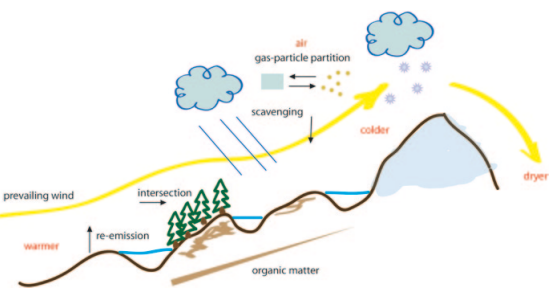
\includegraphics[width=0.82\textwidth]{figures/imgs/TransportMech.png}
            \caption{Conceptual pathways for atmospheric transport and deposition of contaminants in mountainous terrain, including precipitation scavenging, air--surface exchange, and elevation-dependent environmental conditions. Reproduced or adapted from the source discussed by Catalan~\cite{Catalan2015}; confirm the original figure attribution.}
            \label{fig:TransportMechanism}
        \end{figure}
        }{%
        % TODO: Restore figures/imgs/TransportMech.png to display the transport figure.
        }

    \subsection{High-Altitude and Remote Surface-Water Environments}\label{subsec:high-altitude-environments}

        % Remote, high-altitude environments provide useful settings for studying the distribution of environmental contaminants. Locations in the project's research context include Mount Everest, Mount Kilimanjaro, the Qinghai--Tibetan Plateau, and associated surface-water environments. Snow, precipitation, and surface water can provide evidence of atmospheric transport and deposition. Remoteness does not guarantee isolation from human-associated chemicals.
        % This project uses existing environmental HRMS data; sample collection is not itself a contribution of this thesis. The origins, sample types, and analytical details of the datasets used in the software evaluation will be documented in Chapter~2.
        % TODO: Add findings and citations from primary studies relevant to the actual
        % datasets. Do not imply that every cited location is represented in the data.

        High-altitude regions offer valuable settings for examining contaminant transport because their climatic conditions can favor deposition, seasonal storage, and subsequent redistribution of chemicals. Mountain snow and ice may temporarily retain atmospheric contaminants, and melting can transfer some of these substances into downstream waters. The timing and magnitude of release depend on snowpack processes and the properties of the chemicals involved~\cite{Herbert2006,Meyer2008}. Such pathways matter for interpreting surface-water samples, but the detection of a feature alone does not establish its ecological effect or the extent of exposure to organisms.

        Research on mountainous environments has documented persistent organic contaminants and other human-associated chemicals in regions that are geographically distant from major industrial centers~\cite{Daly2005,Xu2011,WangCong2019}. Studies of the Qinghai--Tibetan Plateau also illustrate that spatial patterns of contamination can be influenced by human activity within a highland basin, not solely by long-range atmospheric transport~\cite{Ma2025}. Consequently, these environments should be treated as chemically informative rather than assumed to be free of local sources. Tourism, settlement, transportation, and regional activities may contribute alongside atmospheric inputs, depending on the location and compound.

        Cold trapping is one explanation for the accumulation of particular semivolatile contaminants in mountainous environments. As air temperatures decrease with elevation, some compounds partition more readily into cooler environmental compartments. Seasonal changes can then modify the balance between deposition and re-emission. These exchanges provide a conceptual explanation for how contaminants can be redistributed; they are not direct measurements of the samples analyzed in this thesis~\cite{Daly2005,Herbert2006}.

        \IfFileExists{figures/imgs/Daly_SVOCs.png}{%
        \begin{figure}[htbp]
            \centering
            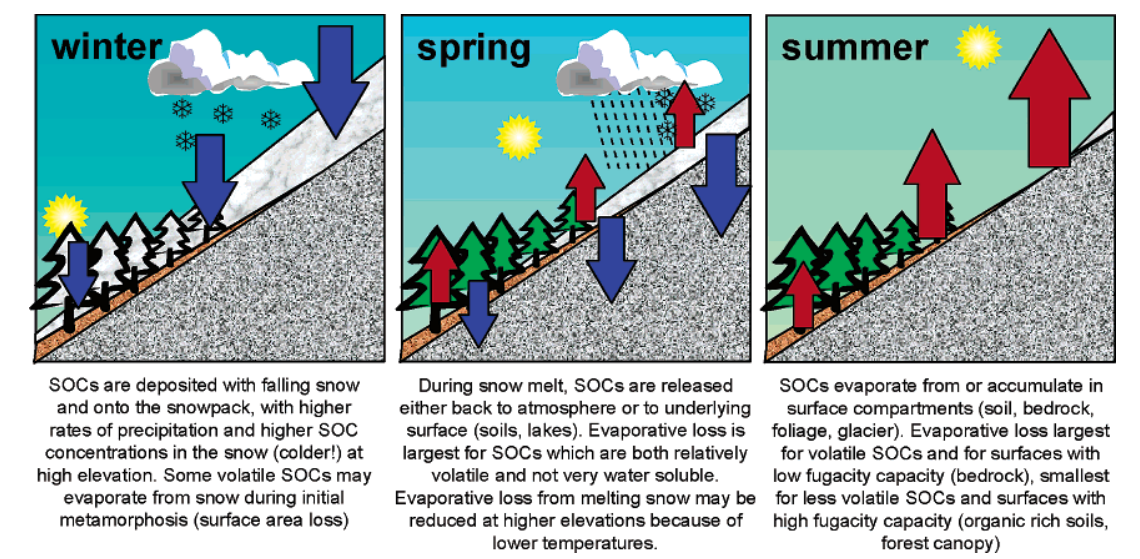
\includegraphics[width=0.78\textwidth]{figures/imgs/Daly_SVOCs.png}
            \caption{Illustration of seasonal air--surface exchange processes affecting semivolatile organic contaminants along a mountain slope. From the discussion of organic contaminants in mountains by Daly and Wania~\cite{Daly2005}; verify reproduction or adaptation permissions.}
            \label{fig:AirSurfaceExchange}
        \end{figure}
        }{%
        % TODO: Restore figures/imgs/Daly_SVOCs.png to display the seasonal exchange figure.
        }

        The published mountain literature provides context for the environmental samples considered in this project. Daly and Wania reviewed studies of persistent organic contaminants at mountain locations and the factors affecting their transport and retention~\cite{Daly2005}. The compilation previously reproduced in the Junior I.S. as a figure is useful as evidence of the range of mountain sites and chemical classes investigated; it should not be described as a plot of contaminant concentrations because it summarizes studies and sampling information rather than presenting a common quantitative scale.

        \IfFileExists{figures/imgs/DalyData.png}{%
        \begin{figure}[htbp]
            \centering
            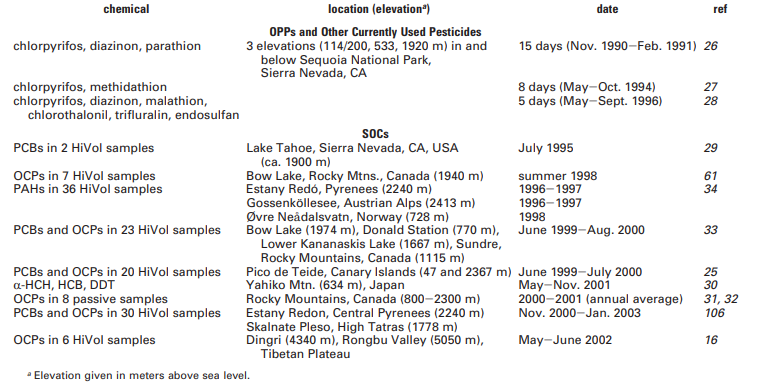
\includegraphics[width=0.92\textwidth]{figures/imgs/DalyData.png}
            \caption{Summary of selected mountain-air contaminant investigations, including reported chemical classes, study locations, and sampling periods, as compiled by Daly and Wania~\cite{Daly2005}. This is a study-summary table, not a comparison of measured concentrations. Verify the original figure attribution.}
            \label{fig:MountainStudies}
        \end{figure}
        }{%
        % TODO: Restore figures/imgs/DalyData.png to display the mountain study summary.
        }

        The present project is motivated by environmental HRMS datasets associated with remote and high-altitude locations, including the Himalayas, Mount Kilimanjaro, and the Qinghai--Tibetan Plateau. These locations provide a chemical context in which both previously recognized contaminants and unannotated features are of interest. The exact samples, matrices, collection locations, and data subsets included in the software evaluation will be specified in Chapter~2. No claim is made here that every location mentioned in the literature is represented in the dataset used for the final case studies.

    \subsection{Previous Wooster Research and the Identification Gap}\label{subsec:wooster-research-gap}

        % Previous research associated with the College of Wooster has investigated organic contaminants in remote and high-altitude environmental samples. This work provides the chemical and analytical context for the current project. Even when LC-HRMS detects features of interest, not every feature can be assigned confidently to a specific compound. A feature may have accurate-mass, retention-time, isotope, or MS/MS information without a confirmed chemical identity.
        % The gap is both chemical and computational. Chemically, researchers need ways to prioritize and interpret features that lack confident identifications. Computationally, they need tools that allow spectral relationships and associated metadata to be examined consistently. This thesis addresses the computational part of that problem while using environmental data to demonstrate how the workflow can support chemical investigation.
        % TODO: Cite specific Wooster studies and distinguish prior researchers' work
        % from analyses performed as part of this thesis.

        Previous work associated with the College of Wooster provides a direct foundation for this study. Fan's undergraduate research investigated suspect screening and semi-quantification of organic contaminants in snow and water from the Qinghai--Tibet Plateau and other high-mountain regions~\cite{Wenkai}. Related research involving Wooster investigators has applied LC-HRMS suspect screening to pesticides in rain and snow, as well as NTA and suspect screening to organic contaminants in temperate snowfall~\cite{Gray2022,NinoSuastegui2025}. These studies are not interchangeable: the temperate precipitation investigations demonstrate analytical approaches, while Fan's work is more directly connected to the remote high-altitude samples motivating this project.

        The identification gap arises because feature detection can yield more information than reference-based annotation can explain. Accurate mass, retention time, isotope information, and MS/MS spectra can be available for a detected feature even when its chemical structure remains uncertain. An unannotated feature may represent a chemical absent from the library, a feature with insufficient-quality evidence, or another analytical signal requiring additional interpretation. It should not automatically be described as a new contaminant or a transformation product~\cite{Manz2023,Schulze2020,Schymanski2014}.

        This distinction defines the need for both chemistry and computer science in the current work. From the chemistry perspective, researchers need to organize evidence and prioritize features that merit further investigation. From the computational perspective, they need to calculate spectral relationships consistently, retain the information behind those relationships, and navigate the resulting network without losing the connection to the original data. The purpose of the new software is to support this investigative process, not to replace confirmatory chemical analysis.

\section{LC-HRMS, Suspect Screening, and Non-Targeted Analysis}\label{sec:lc-hrms}

    \subsection{LC-HRMS and Tandem Mass Spectrometry}\label{subsec:lc-hrms-msms}

        % Liquid chromatography separates components of a sample before they enter a mass spectrometer. High-resolution mass spectrometry measures ions with high mass accuracy and provides information used to characterize molecular features. In tandem mass spectrometry (MS/MS), selected precursor ions are fragmented and the resulting product-ion spectra provide additional evidence about molecular structure. These data support chemical annotation and comparison, but their interpretation depends on data quality and available reference information.
        % TODO: Describe the actual instrument, chromatography, ionization modes, and
        % acquisition conditions in Chapter 2 after checking laboratory records.

        Liquid chromatography separates components of a sample before mass-spectrometric detection, helping resolve some of the complexity of environmental mixtures. High-resolution mass spectrometry measures ions with sufficient mass accuracy to support candidate elemental compositions and other forms of chemical investigation. Depending on the acquisition and processing methods, an LC-HRMS feature can be characterized by a mass-to-charge ratio ($m/z$), retention time, signal intensity, and additional evidence such as an isotope pattern. These attributes are useful for organizing a dataset, but they do not necessarily determine a unique chemical structure~\cite{Manz2023,Kind2018}.

        Tandem mass spectrometry provides another source of information by selecting precursor ions and recording the product ions generated during fragmentation. MS/MS patterns can assist in distinguishing candidates, comparing features, and searching spectral libraries. Their interpretation depends on acquisition conditions, spectral quality, and the reference data available for comparison~\cite{Kind2018,Hupatz2025}. The specific LC-HRMS instrumentation, ionization modes, acquisition strategy, and upstream processing steps associated with the datasets used in this thesis are documented in Chapter~2 rather than assumed from the general analytical literature.

    \subsection{Molecular Features Versus Identified Compounds}\label{subsec:features-compounds}

        % A molecular feature is an observed signal characterized by analytical attributes such as mass-to-charge ratio, retention time, and, when available, isotope or MS/MS information. A feature should not automatically be treated as a confirmed compound. Adduct formation, in-source fragmentation, isomers, incomplete spectra, and limited reference information can complicate interpretation.
        % This thesis uses the term \emph{feature} for detected signals whose chemical identities have not been confirmed. The term \emph{compound} is reserved for cases where the evidence supports that terminology. Network connections and candidate annotations are evidence to investigate, not substitutes for appropriate chemical confirmation.

        A \emph{molecular feature} is an analytical observation rather than a confirmed chemical identity. Multiple observed signals can arise from a single substance through different adducts, isotopes, or fragments, while different substances can also produce overlapping or difficult-to-distinguish signals. For this reason, a feature count is not equivalent to a count of unique contaminants. Likewise, a spectral library match or a relationship to an annotated neighbor does not automatically justify calling an unknown feature an identified compound~\cite{Manz2023,Schymanski2014}.

        Confidence in a chemical assignment should be communicated in relation to the supporting evidence. Schymanski and colleagues proposed a framework for reporting confidence levels in HRMS-based small-molecule identification, ranging from confirmed structures to less specific candidate or formula-level information~\cite{Schymanski2014}. Within this thesis, \emph{feature} is used when identity has not been established, while \emph{candidate annotation} or \emph{tentative identification} describes an assignment supported by incomplete evidence. A confirmed identification requires the appropriate confirmation criteria, such as comparison with an authentic reference standard when relevant. The confidence associated with individual case-study features will be stated rather than inferred from network appearance.

    \subsection{Suspect Screening and Non-Targeted Analysis}\label{subsec:suspect-nta}

        % Targeted analysis focuses on a predefined set of compounds. Suspect screening examines data for compounds on a suspect list, including compounds that may not be part of a conventional targeted method. Non-targeted analysis (NTA) aims to detect and investigate a broader range of chemical features without restricting the analysis to a fixed list of target compounds.
        % These approaches are complementary. Suspect screening can investigate compounds for which there is a prior reason to look, while NTA can retain information about features not anticipated in advance. Neither approach guarantees that every detected feature can be identified. Candidate assignments must be evaluated against available mass, retention-time, isotope, and fragmentation evidence, as applicable.

        Targeted analysis begins with a defined set of analytes and methods selected to measure them. It is valuable for questions concerning known chemicals, but its scope is constrained by the compounds included in the method. Suspect screening broadens that scope by examining acquired data for chemicals of prior interest, often using information from candidate lists and available analytical evidence. NTA takes a wider approach by retaining and investigating features without requiring that every candidate be specified before data acquisition~\cite{Manz2023,Schulze2020}.

        These strategies are complementary rather than mutually exclusive. Suspect screening can prioritize features associated with known environmental concerns, while NTA can reveal additional signals that do not match the current suspect list. Published studies of pesticides in rain and snow and of broader organic chemical mixtures in snowfall demonstrate the value of these approaches in environmental LC-HRMS workflows~\cite{Gray2022,NinoSuastegui2025}. At the same time, an expanded set of detected features creates a larger interpretation problem: researchers must decide which signals are chemically meaningful and what evidence supports each possible assignment.

        The term \emph{exposome} provides a broader context for this challenge by referring to the totality of exposures across time, including chemical exposures. NTA and suspect screening can contribute information about portions of this chemical landscape, but no single analytical dataset measures the entire exposome~\cite{Manz2023}. For the present project, the more immediate objective is to investigate environmental feature relationships in the available data, not to quantify total exposure or infer health effects.

    \subsection{Limitations of Current Identification Approaches}\label{subsec:identification-limitations}

        % Reference databases and spectral libraries are incomplete. A detected feature may not have a suitable reference spectrum, and different structures can sometimes produce similar or partially overlapping fragmentation patterns. Data quality, acquisition conditions, and processing choices can also affect the evidence available for interpretation.

        % Identifying and prioritizing unknown features therefore requires researchers to combine different types of evidence and preserve uncertainty in their conclusions. A computational tool can help organize data and make relationships easier to inspect, but it should not convert a similarity score or network connection into an unsupported claim of chemical identity.
        Even when high-resolution data are available, many features remain without confident annotations. Reference databases may not contain a relevant chemical or its spectrum, experimental conditions may differ from those used to generate a library spectrum, and the available MS/MS data may be incomplete or ambiguous. Reviews of environmental NTA and computational structural annotation describe these constraints and emphasize the importance of quality control and careful reporting~\cite{Schulze2020,Hupatz2025,Fisher2022}.

        The consequence is a gap between \emph{detection} and \emph{interpretation}. Increasing the number of observed features does not necessarily increase the number of confidently identified substances. Additional computational methods can help organize the evidence, identify promising comparisons, and prioritize follow-up work, but they must preserve uncertainty instead of presenting every computational association as a chemical conclusion. Molecular networking is one such method, and its theoretical basis is developed in the following section.

\section{Molecular Networking and Theoretical Foundations}\label{sec:molecular-networking}

    \subsection{MS/MS Fragmentation and Spectral Similarity}\label{subsec:fragmentation-similarity}

        % MS/MS spectra represent product ions generated when a precursor ion fragments under specified conditions. Related molecules may share some fragments or fragmentation patterns, so comparing spectra can provide clues about structural similarities. The strength of these inferences depends on spectrum quality, the comparison method, and the chemical context.
        % Spectral similarity is best treated as a way to prioritize and explore possible relationships. It is not, on its own, definitive evidence that two features represent the same molecule or lie on a specific transformation pathway.

        A tandem mass spectrum records product ions and their intensities after a precursor ion undergoes fragmentation. Structurally related molecules can share fragments or fragmentation pathways, which creates a basis for comparing their spectra. Nevertheless, the relationship between structure and spectral similarity is not one-to-one. Different compounds may share characteristic fragments, and the same compound may yield different relative intensities under different acquisition conditions. Spectral comparisons are therefore useful evidence for exploratory analysis, not direct proof of identity~\cite{Wang2016,Bittremieux2022}.

        In a molecular network, this comparison becomes a relationship between features. An annotated feature may provide context for neighboring features, including those that have no direct library match. Such proximity can help prioritize a chemical family or candidate structure for further investigation, but any proposed relationship must be evaluated against the available fragmentation data, precursor information, and independent chemical evidence~\cite{Schmid2021,Ernst2019,Schymanski2014}.

    \subsection{Cosine Similarity and Molecular-Network Construction}\label{subsec:cosine-network}

        % A spectral similarity score quantifies the correspondence between two spectra under a specified comparison procedure. Cosine similarity is one common approach. After spectra are represented and peaks are matched according to defined rules, the score summarizes alignment between the resulting spectral vectors. The score depends on implementation choices such as peak matching, mass tolerances, preprocessing, and filtering.
        % In a molecular network, each node represents a molecular feature and an edge represents a relationship that meets the selected similarity criteria. Edge weights or labels can retain the similarity score so researchers can inspect the computational relationship. Thresholds affect the resulting graph: stricter criteria may remove weaker connections, while more permissive criteria may create a denser network. The chosen settings and their rationale should therefore be documented.
        % TODO: Add the exact similarity implementation, peak-matching rules, and
        % thresholds once finalized. Detailed implementation belongs in Chapter 2.

        Cosine similarity is a common method for measuring agreement between represented mass spectra. After an appropriate peak-matching or alignment procedure, spectra can be expressed as nonnegative intensity vectors $\mathbf{x}$ and $\mathbf{y}$. Their cosine similarity is
        \begin{equation}
            \operatorname{cos}(\mathbf{x},\mathbf{y})
            = \frac{\mathbf{x}\cdot\mathbf{y}}
            {\lVert\mathbf{x}\rVert_2\,\lVert\mathbf{y}\rVert_2}.
            \label{eq:spectral-cosine}
        \end{equation}
        For nonnegative intensity vectors, values closer to one indicate greater agreement under the selected representation and matching procedure. The score is meaningful only in the context of those choices. Peak matching, mass tolerances, intensity treatment, minimum matching requirements, and any modified-cosine or neutral-loss logic can change the comparisons and the resulting network~\cite{Bittremieux2022,DallaValle2025}.

        The score is not itself an edge. A molecular-networking workflow applies additional rules to determine which pairwise similarities are retained as connections, such as a minimum score or other filters. Different rules can produce different network densities and connected components from the same spectra. Consequently, a reproducible workflow must document its comparison method and parameter values. Chapter~2 describes the actual algorithm and edge-selection rules implemented in this project; Equation~\ref{eq:spectral-cosine} establishes the general mathematical foundation rather than claiming that a particular implementation has already been validated.

    \subsection{Graph Theory: Nodes, Edges, and Connected Components}\label{subsec:graph-theory}

        % Graph theory provides a formal way to represent relationships among objects. In molecular networking, nodes represent features and edges represent the spectral relationships retained by the workflow. A connected component is a set of nodes connected through paths in the graph. Isolated nodes have no retained edges under the selected network criteria.
        % These structures help summarize and navigate relationships in a dataset. However, a connected component should not automatically be interpreted as one chemical family, and an edge should not be treated as proof of shared identity or a reaction pathway. Interpretation requires considering the graph alongside spectral evidence, metadata, annotations, and analytical limitations.

        A molecular network can be represented as a graph $G=(V,E)$, where $V$ is the set of nodes representing analytical features and $E$ is the set of retained spectral relationships. An edge may carry a similarity score or other metadata describing the evidence for the relationship. This representation provides a computational structure for organizing large sets of pairwise comparisons and exploring groups of related observations~\cite{Barabasi2016,Wang2016}.

        A \emph{connected component} is a maximal set of nodes linked through paths in the graph. Components can help organize a network into smaller groups for inspection, while isolated nodes represent features without retained edges under the chosen criteria. These are graph properties, not chemical classifications. In particular, two features in the same component may be connected only indirectly, and membership in a component does not establish a shared molecular formula, common source, or transformation pathway.

    \subsection{Network Visualization and Interpretation}\label{subsec:network-visualization}

        % Network visualization can help researchers inspect complex relationships that may be difficult to explore in a table alone. Selecting nodes and edges, viewing feature metadata, examining similarity values, and filtering the network can connect the overall graph to the underlying chemical evidence. Visual encodings should communicate meaningful properties without implying more certainty than the data support.
        % The interface is most useful when users can move between the network-level view and the evidence behind a connection. Users should be able to inspect which features are connected, why an edge is present under the selected criteria, and what information is available about the features. Important settings and data provenance should be accessible enough to support repeatable analysis.

        Visualization translates the graph into an interface that chemists can explore. A useful view should allow researchers to identify features and their connections, inspect similarity scores, and retrieve the metadata or spectra associated with a selected node or edge. Color, size, layout, and filtering can make patterns easier to see, but these visual choices must be defined so that they do not imply greater chemical certainty than the underlying data justify. Research on interactive graph exploration supports the importance of connecting overview visualizations with inspectable data and user tasks~\cite{Pienta2015,Jacomy2014}.

        The distinction between a graphical display and a scientific workflow is important for this project. A static image of a network may communicate broad structure, but it cannot by itself establish which source records produced an edge or whether an analysis can be repeated with the same parameters. The proposed interface therefore emphasizes the relationship between visual elements, underlying feature data, and the computations used to generate connections. The implemented interactions and their evaluation will be described in Chapters~2 and~3.

    \subsection{Limitations of Spectral Similarity as Evidence of Chemical Identity}\label{subsec:spectral-limitations}

        % A high spectral similarity score indicates agreement under the selected computational comparison; it does not independently establish molecular identity. Similar spectra can arise for different structures, and structurally related compounds can produce different spectra under different conditions. Missing or low-quality MS/MS data may also weaken or prevent meaningful comparisons.
        % The software developed in this project is intended to support exploration of evidence rather than replace expert chemical judgment or confirmatory experiments. Where reference standards or other appropriate confirmation are absent, the thesis will distinguish tentative annotations and possible relationships from confirmed identifications.

        Spectral similarity can support hypotheses about structural relationships, but it cannot independently confirm the identity of an unknown compound. Shared fragment ions may arise from different structures, and changes in collision energy, ionization, and spectral quality can alter the apparent similarity between spectra~\cite{Bittremieux2022,Hupatz2025}. Likewise, a mass difference between two connected features does not, without further evidence, demonstrate that one is a transformation product of the other.

        This limitation shapes both the software design and the chemistry case studies. The network should make comparisons inspectable and preserve annotation confidence, while interpretation should distinguish observations, tentative hypotheses, and confirmed assignments. The intended benefit is more informed prioritization of unknown features, not an automatic conversion of spectral relationships into definitive chemical identifications~\cite{Schymanski2014,Chao2025}.

\section{Existing Software and Research Gap}\label{sec:existing-software}

    \subsection{MS-DIAL and GNPS in the Existing Workflow}\label{subsec:msdial-gnps}

        % The existing research workflow uses MS-DIAL for upstream processing of mass-spectrometry data and molecular-networking tools such as the Global Natural Products Social Molecular Networking platform (GNPS) to explore spectral relationships. These tools address different stages of the workflow: processing software prepares and organizes analytical data, while molecular-networking software represents relationships among features.
        % This project builds on that workflow rather than assuming that any one tool is universally unsuitable. The relevant question is whether the workflow used for the College of Wooster's environmental HRMS research meets practical requirements for data handling, network inspection, reproducibility, and interpretation.
        % TODO: Verify tool versions, export formats, and workflow steps against
        % project records. Describe only limitations that were observed or documented.

        Mass-spectrometry analysis typically involves multiple computational stages. In the Wooster research context, MS-DIAL is used for upstream data processing and feature-level outputs, while molecular-networking approaches associated with the Global Natural Products Social Molecular Networking platform (GNPS) provide methods for organizing MS/MS relationships~\cite{Tsugawa2015,Wang2016,Schmid2021}. These tools address different analytical tasks and have established value in their respective areas. The objective of this thesis is not to suggest that the existing platforms are universally inadequate, nor to replace every stage of LC-HRMS data processing.

        Instead, the project focuses on the transition from processed analytical data to a molecular network that can be explored and reproduced in the local research workflow. The input and export formats, metadata requirements, and comparison methods at this boundary affect whether the results remain interpretable after they leave the original processing software. The specific versions and settings used for the project data will be documented in Chapter~2.

    \subsection{Documented Limitations in the Wooster Research Workflow}\label{subsec:workflow-limitations}

        % The motivation for this project includes workflow difficulties reported during local molecular-networking work, particularly around preserving work and reliably saving or exporting results. These concerns should be described as observed or reported issues in this specific research context, not as a general claim that GNPS or other existing platforms fail for all users.
        % The project will translate relevant research needs into explicit software requirements. These may include dependable input handling, inspectable node and edge information, links between network elements and chemical metadata, and clear behavior when saving or exporting results. The final requirements should reflect documented needs and features actually implemented and evaluated.

        The software-development motivation arose from difficulties reported in local molecular-networking work, particularly around saving, retaining, or exporting analyses and results. Such problems matter because a network is useful for research only when its underlying data, parameter choices, and interpretations can be revisited. These concerns are presented as local workflow requirements that motivate this project, not as evidence that GNPS necessarily behaves the same way for every user or deployment.

        A reliable workflow must also support the scientific interpretation of its outputs. A chemist examining a connected pair of features needs access to the corresponding identifiers, spectra, annotations, and similarity evidence. Without those links, an attractive visualization may be difficult to verify or use in subsequent analysis. Reproducibility likewise depends on retaining input provenance, computational parameters, and sufficient documentation to repeat the workflow~\cite{Wilson2017,Pienta2015}. The particular requirements adopted for this project will be made explicit and evaluated rather than assumed to have been satisfied.

    \subsection{The Need for Software Designed Around Chemists' Needs}\label{subsec:chemist-centered-software}

        % Molecular-networking software must do more than generate a graph. It should help users move between a network-level view and the underlying evidence, understand how connections were calculated, and preserve the information needed to reproduce an analysis. The interface should make important details accessible without requiring users to reconstruct the workflow from separate files or undocumented steps.
        % This project treats software reliability and usability as research concerns alongside the chemical application. The proposed contribution is a workflow and interface tailored to the current environmental HRMS research context, evaluated through computational tests and case studies using real data. Its success will be assessed based on implemented functionality and measured results rather than assumed in advance.

        The research gap is therefore both analytical and computational. Incomplete reference coverage leaves many environmental HRMS features unidentified, while a practical molecular-networking workflow must make spectral comparisons, graph relationships, and supporting metadata accessible to researchers. Existing tools demonstrate the value of molecular networking, but the requirements of a particular laboratory workflow still need to be defined, implemented, and tested~\cite{Wang2016,Schmid2021,Chao2025}.

        This thesis approaches software as a scientific research instrument rather than merely a way to display a network. The proposed contribution is a workflow and interface tailored to Wooster's environmental HRMS context, with attention to computational correctness, reproducibility, data handling, and the interpretability of network relationships. Its value will be assessed through software evaluation and chemical case studies. The chemistry contribution concerns what can reasonably be learned or prioritized from the environmental data; the computer science contribution concerns how reliably and transparently the software supports that investigation.

\section{Research Question and Specific Aims}\label{sec:research-question}

    The central research question is:

    \begin{quote}
    What computational workflow and interface are needed to make molecular networking reliable, reproducible, and useful for Wooster's environmental HRMS research?
    \end{quote}

    The project addresses this question through four aims:

    \begin{enumerate}
        \item \textbf{Define the chemistry and data requirements.} Identify the analytical data, metadata, and evidence needed to construct and interpret molecular networks for the environmental HRMS research context.
        \item \textbf{Develop an end-to-end molecular-networking workflow.} Implement a workflow that processes supported input data, compares MS/MS spectra, constructs a network, and allows users to inspect network elements and associated chemical information.
        \item \textbf{Evaluate computational correctness, reproducibility, performance, and workflow usefulness.} Test calculations, input handling, graph construction, repeatability, performance, and relevant user-facing tasks using documented evaluation methods.
        \item \textbf{Apply the software to environmental HRMS case studies.} Use selected environmental data to examine annotated and unidentified features, describe relationships supported by the evidence, and identify remaining uncertainties.
    \end{enumerate}

\section{Project Scope and Thesis Contributions}\label{sec:scope-contributions}

    \subsection{Project Scope}\label{subsec:project-scope}

        This project focuses on computational support for molecular networking using existing environmental HRMS data. It includes defining data requirements, implementing and testing the network workflow, designing an interface for inspecting features and spectral relationships, and applying the software to selected chemical case studies. The specific input formats, data-processing assumptions, software features, and evaluation procedures will be defined in Chapter~2.

        The project does not assume that a network alone can confirm the identity of unknown compounds, prove chemical transformation pathways, or replace reference standards and other confirmatory methods. Software development alone also does not establish the environmental source, toxicity, or ecological effect of a detected feature. Claims in the chemical case studies will be limited to what the available analytical data and supporting evidence justify.

    \subsection{Expected Computer Science Contributions}\label{subsec:cs-contributions}

        The Computer Science contribution is the design, implementation, and evaluation of a molecular-networking workflow and interface for the stated research context. The contribution will be documented through the software architecture, similarity and graph-construction methods, interface behavior, input validation, testing, and reproducibility practices. Chapter~3 will report what was implemented and how it performed under the evaluation procedures.

    \subsection{Expected Chemistry Contributions}\label{subsec:chemistry-contributions}

        The Chemistry contribution is the application of the workflow to environmental HRMS data to investigate spectral relationships among annotated and unidentified molecular features. The case studies will describe the evidence available for selected features, explain how network relationships may help prioritize further investigation, and state the remaining limitations. Tentative network relationships will not be presented as confirmed chemical identifications.

    \subsection{Organization of the Thesis}\label{subsec:thesis-organization}

        Chapter~2 describes the research design, environmental datasets and analytical methods, upstream processing, software requirements and implementation, network construction, and evaluation procedures. Chapter~3 presents the dataset summary, software implementation results, computational validation, performance and workflow evaluation, network characteristics, and chemical case studies. Chapter~4 interprets the computational and chemical findings, discusses design trade-offs and limitations, and considers implications for future environmental HRMS research. Chapter~5 summarizes the contributions, answers the central research question, and identifies future directions.

%!TEX root = ../main.tex

\chapter{Methodology, Research Design, and Software Development}\label{ch:methodology}

  \section{Overall Research Design and Workflow}\label{sec:research-design}
  % Describe the overall research approach and data flow.
  % Explain the relationship between the chemistry and computational components.
  % Introduce the research datasets and evaluation strategy.

  \section{Environmental Samples and Chemistry Experimental Methods}\label{sec:environmental-samples}
  % Describe sample origins, locations, and sample types.
  % Document instrumentation and analytical conditions.
  % Describe LC-HRMS and MS/MS acquisition.
  % Explain positive- and negative-ion modes, where applicable.
  % Clarify which experimental work was performed by previous researchers.

  \section{Upstream Data Processing and Chemical Annotation}\label{sec:data-processing}
  % Document MS-DIAL processing and version.
  % Describe feature detection, alignment, and spectral exports, as applicable.
  % Explain data-quality checks and inclusion criteria.
  % Describe suspect screening, candidate annotations, and metadata.
  % Discuss identification confidence and limitations.

  \section{Software Requirements and System Architecture}\label{sec:software-architecture}
  % Define functional and nonfunctional requirements.
  % Document supported input formats and validation.
  % Describe system modules and data flow.
  % Explain data structures and metadata representation.
  % Describe reproducibility and provenance.

  \section{Spectral Comparison and Similarity Calculation}\label{sec:spectral-similarity}
  % Describe spectrum representation and preprocessing.
  % Explain peak matching and mass tolerances.
  % Document the cosine similarity implementation.
  % Define edge thresholds and computational considerations.
  % Explain handling of missing, incomplete, or unusable spectra.

  \section{Molecular-Network Construction}\label{sec:network-construction}
  % Describe node and edge representation.
  % Define similarity thresholds and graph filtering.
  % Explain connected components and isolated features.
  % Describe how network elements link to chemical metadata.

  \section{User Interface Design and Interaction}\label{sec:interface-design}
  % Describe network layout and visual encodings.
  % Explain node and edge selection.
  % Document feature metadata and similarity inspection.
  % Describe filtering, navigation, and network exploration.
  % Document saving, exporting, and persistence, where implemented.
  % Explain design decisions informed by chemist workflows.

  \section{Software Implementation and Reproducibility}\label{sec:implementation}
  % Document programming languages, libraries, and dependencies.
  % Describe modular design, version control, and documentation.
  % Explain error handling and logging.
  % Describe configuration, parameter recording, and reproducible execution.

  \section{Software Evaluation and Testing Methods}\label{sec:evaluation-methods}
  % Describe unit, integration, and end-to-end tests.
  % Explain reference calculations for similarity validation.
  % Document graph-construction correctness checks.
  % Describe repeated-run reproducibility tests.
  % Define runtime and scalability measurements.
  % Explain interface and workflow task evaluation.

  \section{Chemical Case-Study Design}\label{sec:case-study-design}
  % Explain the selection of representative environmental samples.
  % Define criteria for selecting samples, features, and network clusters.
  % Describe the use of existing annotations and spectral evidence.
  % Explain interpretation of known and unidentified features.
  % Define criteria for limiting chemical claims.

%!TEX root = ../main.tex

\chapter{Results and Data Analysis}\label{ch:results}

  \section{Environmental Dataset and Feature Summary}\label{sec:dataset-summary}
  % Describe dataset characteristics and sample coverage.
  % Report input features and usable MS/MS spectra.
  % Summarize available annotations, exclusions, and data limitations.

  \section{Software Implementation Results}\label{sec:implementation-results}
  % Describe the completed workflow and supported functionality.
  % Present the implemented architecture and interface.
  % Include representative input-to-network examples.

  \section{Computational Correctness and Validation}\label{sec:correctness-validation}
  % Compare similarity calculations against reference values.
  % Report input-validation and error-handling results.
  % Present network-construction test results.
  % Report reproducibility and persistence results.

  \section{Software Performance and Workflow Evaluation}\label{sec:performance-results}
  % Report runtime and memory use, where measured.
  % Compare performance across tested dataset sizes.
  % Present interface and workflow task results.
  % Summarize requirements met, partially met, or unmet.

  \section{Molecular-Network Structure and Characteristics}\label{sec:network-results}
  % Report nodes, edges, connected components, and isolated features.
  % Analyze similarity-score distributions.
  % Present the effects of thresholds and filtering, where evaluated.

  \section{Chemical Case Study 1: Annotated Molecular Features}\label{sec:annotated-features}
  % Introduce the selected network and chemical context.
  % Present spectral relationships and available annotations.
  % Discuss the strength of the supporting evidence.

  \section{Chemical Case Study 2: Unidentified Molecular Features}\label{sec:unidentified-features}
  % Present selected unknown features or network clusters.
  % Examine relationships to annotated or other unidentified features.
  % Discuss potential chemical relationships and unresolved questions.

  \section{Summary of Principal Results}\label{sec:principal-results}
  % Synthesize the strongest computational and chemical findings.

%!TEX root = ../main.tex

\chapter{Discussion}\label{ch:discussion}

    \section{Interpretation and Integration of Results}\label{sec:results-integration}
    % Answer the central research question using both result sets.
    % Explain how chemistry informed software design and evaluation.
    % Discuss how the software supported chemical investigation.

    \section{Computational Contributions and Design Trade-Offs}\label{sec:computational-contributions}
    % Discuss reliability, correctness, reproducibility, and usability.
    % Evaluate strengths and weaknesses of algorithms and architecture.
    % Compare results with intended requirements and existing workflows.

    \section{Chemical Significance and Comparison with Literature}\label{sec:chemical-significance}
    % Interpret the chemical case-study findings.
    % Relate findings to existing environmental chemistry research.
    % Discuss what molecular networking reveals about unknown features.
    % Explain limits on claims about identity and transformation products.

    \section{Study and Implementation Limitations}\label{sec:limitations}
    % Discuss analytical and data-quality limitations.
    % Evaluate computational and scalability limitations.
    % Discuss visualization and workflow limitations.
    % Explain evaluation constraints and limits on generalization.

    \section{Implications for Future Environmental HRMS Research}\label{sec:future-implications}
    % Explain how the workflow may support future Wooster projects.
    % Identify additional data, validation, and software capabilities needed.

%\input{chapters/chapter4}
%\input{chapters/chapter5}
%\input{chapters/chapter6}
%\input{chapters/chapter7}
%!TEX root = ../main.tex

\chapter{Conclusions and Future Work}\label{ch:conclusions}

    \section{Summary of the Research}\label{sec:research-summary}
    % Revisit the environmental problem, objectives, and approach.

    \section{Principal Computer Science Contributions}\label{sec:cs-contributions}
    % Summarize the implemented workflow and evaluation findings.

    \section{Principal Chemistry Contributions}\label{sec:chemistry-contributions}
    % Summarize the supported chemical findings and their significance.

    \section{Answer to the Central Research Question}\label{sec:research-question-answer}
    % State what the project demonstrated and what remains unresolved.

    \section{Future Work}\label{sec:future-work}
    % Discuss additional validation and environmental datasets.
    % Propose software improvements and further chemical investigation.

    \section{Final Remarks}\label{sec:final-remarks}
    % Conclude with the project's contribution to computational chemistry.


%%%%%%%%%%%%%%%%%%%%%%%%%%%%%%%%%%%%%%%%%%%%%%%%%%%%%%%
%
%  This section starts the back matter. The back matter includes appendices, indicies, and the
%  bibliography
%
%%%%%%%%%%%%%%%%%%%%%%%%%%%%%%%%%%%%%%%%%%%%%%%%%%%%%%%

\backmatter

%%!TEX root = ../main.tex
%%%%%%%%%%%%%%%%%%%%%%%%%%%%%%%%%%%%%%%%%%%%%%%%%%%%%%%%%%%%%%%%
% Contents: Math typesetting with LaTeX
% $Id: math.tex,v 1.3 2005/05/21 02:03:43 jonb Exp $
%%%%%%%%%%%%%%%%%%%%%%%%%%%%%%%%%%%%%%%%%%%%%%%%%%%%%%%%%%%%%%%%%

\chapter{Typesetting Mathematical Formulae}\label{math}
\begin{intro}
  This appendix is taken from \citet{ophs03} under the GNU open-source documentation license. This appendix addresses the main strength
  of \TeX{}: mathematical typesetting. But be warned, this appendix
  only scratches the surface. While the things explained here are
  sufficient for many people, don't despair if you can't find a
  solution to your mathematical typesetting needs here. It is highly likely
  that your problem is addressed in \AmS-\LaTeX{}%
  \footnote{\texttt{CTAN:/tex-archive/macros/latex/packages/amslatex}}
  or some other package.
\end{intro}
  
\section{General}

\LaTeX{} has a special mode for typesetting mathematics\index{mathematics}.
Mathematical text within a paragraph is entered between \verb|\(|\index{\(@\verb+\(+}
and \verb|\)|\index{\)@\verb+\)+}, %$
between \texttt{\$} and \texttt{\$} or between
\verb|\begin{|{math}\verb|}| and \verb|\end{math}|.\index{formulae}

\begin{singlespace}
\begin{example}
Add $a$ squared and $b$ squared 
to get $c$ squared. Or, using 
a more mathematical approach:
$c^{2}=a^{2}+b^{2}$
\end{example}
\end{singlespace}

\begin{singlespace}
\begin{example}
\TeX{} is pronounced as 
$\tau\epsilon$.\\[6pt]
100~m$^{3}$ of water\\[6pt]
This comes from my $\heartsuit$
\end{example}
\end{singlespace}

It is preferable to \emph{display} larger mathematical equations or formulae,
rather than to typeset them on separate lines. This means you enclose them
in \verb|\[| \index{\[@\verb+\[+} and \verb|\]| \index{\]@\verb+\]+} or between
\verb|\begin{|displaymath\index{displaymath}\verb|}| and
  \verb|\end{displaymath}|.  This produces formulae which are not
numbered. If you want \LaTeX{} to number them, you can use the
equation\index{equation} environment.


\begin{singlespace}
\begin{example}
Add $a$ squared and $b$ squared 
to get $c$ squared. Or, using 
a more mathematical approach:
\begin{displaymath}
c^{2}=a^{2}+b^{2}
\end{displaymath}
And just one more line.
\end{example}
\end{singlespace}

You can reference an equation with \ic{label} and \ic{ref}

\begin{singlespace}
\begin{example}
\begin{equation} \label{eq:eps}
\epsilon > 0
\end{equation}
From (\ref{eq:eps}), we gather 
\ldots
\end{example}
\end{singlespace}

Note that expressions will be typeset in a different style if displayed:

\begin{singlespace}
\begin{example}
$\lim_{n \to \infty} 
\sum_{k=1}^n \frac{1}{k^2} 
= \frac{\pi^2}{6}$
\end{example}
\end{singlespace}
\begin{singlespace}
\begin{example}
\begin{displaymath}
\lim_{n \to \infty} 
\sum_{k=1}^n \frac{1}{k^2} 
= \frac{\pi^2}{6}
\end{displaymath}
\end{example}
\end{singlespace}

There are differences between \emph{math mode} and \emph{text mode}. For
example, in \emph{math mode}: 

\begin{enumerate}

\item Most spaces and linebreaks do not have any significance, as all spaces
either are derived logically from the mathematical expressions or
have to be specified using special commands such as \verb|\,| \index{''\,@\verb+\,+}, \ic{quad}, or \ic{qquad}.
 
\item Empty lines are not allowed. Only one paragraph per formula.

\item Each letter is considered to be the name of a variable and will be
typeset as such. If you want to typeset normal text within a formula
(normal upright font and normal spacing) then you have to enter the
text using the \verb|\textrm{...}| commands.
\end{enumerate}


\begin{singlespace}
\begin{example}
\begin{equation}
\forall x \in \mathbf{R}:
\qquad x^{2} \geq 0
\end{equation}
\end{example}
\end{singlespace}

\begin{singlespace}
\begin{example}
\begin{equation}
x^{2} \geq 0\qquad
\textrm{for all }x\in\mathbf{R}
\end{equation}
\end{example}
\end{singlespace}

Mathematicians can be very fussy about which symbols are used:
it would be conventional here to use `blackboard bold\index{blackboard bold}',
bold symbols\index{bold symbols} which is obtained using \ic{mathbb} from the
package \ip{amsfonts} or \ip{amssymb}.

\ifx\mathbb\undefined\else
The last example becomes
\begin{singlespace}
\begin{example}
\begin{displaymath}
x^{2} \geq 0\qquad
\textrm{for all }x\in\mathbb{R}
\end{displaymath}
\end{example}
\end{singlespace}
\fi

\section{Grouping in Math Mode}

Most math mode commands act only on the next character. So if you
want a command to affect several characters, you have to group them
together using curly braces: \verb|{...}|.

\begin{singlespace}
\begin{example}
\begin{equation}
a^x+y \neq a^{x+y}
\end{equation}
\end{example}
\end{singlespace}
 
\section{Building Blocks of a Mathematical Formula}

In this section, the most important commands used in mathematical
typesetting will be described. Take a look at \citet{kd03} for a detailed list of commands for typesetting
mathematical symbols.

\textbf{Lowercase Greek letters\index{Greek letters}} are entered as \verb|\alpha|,
 \verb|\beta|, \verb|\gamma|, \ldots, uppercase letters
are entered as \verb|\Gamma|, \verb|\Delta|, \ldots\footnote{There is no
  uppercase Alpha defined in \LaTeXe{} because it looks the same as a
  normal roman A. Once the new math coding is done, things will
  change.} 

\begin{singlespace}
\begin{example}
$\lambda,\xi,\pi,\mu,\Phi,\Omega$
\end{example}
\end{singlespace}
 
\textbf{Exponents and Subscripts} can be specified using\index{exponent}\index{subscript}
the \verb|^|\index{^@\verb+^+} and the \verb|_|\index{_@\verb+_+} character.

\begin{singlespace}
\begin{example}
$a_{1}$ \qquad $x^{2}$ \qquad
$e^{-\alpha t}$ \qquad
$a^{3}_{ij}$\\
$e^{x^2} \neq {e^x}^2$
\end{example}
\end{singlespace}

The \textbf{square root\index{square root}} is entered as \ic{sqrt}, the
$n^\mathrm{th}$ root is generated with \verb|\sqrt[|$n$\verb|]|. The size of
the root sign is determined automatically by \LaTeX. If just the sign
is needed, use \ic{surd}.

\begin{singlespace}
\begin{example}
$\sqrt{x}$ \qquad 
$\sqrt{ x^{2}+\sqrt{y} }$ 
\qquad $\sqrt[3]{2}$\\[3pt]
$\surd[x^2 + y^2]$
\end{example}
\end{singlespace}

The commands \ic{overline} and \ic{underline} create
\textbf{horizontal lines} directly over or under an expression.
\index{horizontal!line}

\begin{singlespace}
\begin{example}
$\overline{m+n}$
\end{example}
\end{singlespace}

The commands \ic{overbrace} and \ic{underbrace} create
long \textbf{horizontal braces} over or under an expression.
\index{horizontal!brace}

\begin{singlespace}
\begin{example}
$\underbrace{ a+b+\cdots+z }_{26}$
\end{example}
\end{singlespace}

\index{mathematical!accents} To add mathematical accents such as small
arrows or {tilde} signs to variables, you can use the commands
given in \citet{kd03}.  Wide hats and
tildes covering several characters are generated with \ic{widetilde}
and \ic{widehat}.  The \verb|'|\index{'@\verb+'+} symbol gives a
prime\index{prime}.
% a dash is --

\begin{singlespace}
\begin{example}
\begin{displaymath}
y=x^{2}\qquad y'=2x\qquad y''=2
\end{displaymath}
\end{example}
\end{singlespace}

\textbf{Vectors}\index{vectors} often are specified by adding a small
arrow symbol\index{arrow symbols} on top of a variable. This is done with the
\ic{vec} command. The two commands \ic{overrightarrow} and
\ic{overleftarrow} are useful to denote the vector from $A$ to $B$.

\begin{singlespace}
\begin{example}
\begin{displaymath}
\vec a\quad\overrightarrow{AB}
\end{displaymath}
\end{example}
\end{singlespace}

Names of log-like functions are often typeset in an upright
font and not in italic like variables. Therefore \LaTeX{} supplies the
following commands to typeset the most important function names:
\index{mathematical!functions}

\begin{singlespace}
\begin{verbatim}
\arccos   \cos    \csc   \exp   \ker     \limsup  \min   \sinh
\arcsin   \cosh   \deg   \gcd   \lg      \ln      \Pr    \sup
\arctan   \cot    \det   \hom   \lim     \log     \sec   \tan
\arg      \coth   \dim   \inf   \liminf  \max     \sin   \tanh
\end{verbatim}
\end{singlespace}

\begin{singlespace}
\begin{example}
\[\lim_{x \rightarrow 0}
\frac{\sin x}{x}=1\]
\end{example}
\end{singlespace}

For the modulo function\index{modulo function}, there are two commands: \ic{bmod} for the
binary operator ``$a \bmod b$'' and \ic{pmod}
for expressions
such as ``$x\equiv a \pmod{b}$.''

A built-up \textbf{fraction\index{fraction}} is typeset with the
\ic{frac}\verb|{...}{...}| command.
Often the slashed form $1/2$ is preferable, because it looks better
for small amounts of `fraction material.'

\begin{singlespace}
\begin{example}
$1\frac{1}{2}$~hours
\begin{displaymath}
\frac{ x^{2} }{ k+1 }\qquad
x^{ \frac{2}{k+1} }\qquad
x^{ 1/2 }
\end{displaymath}
\end{example}
\end{singlespace}

To typeset binomial coefficients or similar structures, you can use
either the command \linebreak \ic{binom}\{\emph{num}\}\{\emph{denom}\} or \ic{genfrac}\{\emph{ldelim}\}\{\emph{rdelim}\}\{\emph{thickness}\}\{\emph{style}\}\{\emph{num}\}\{\emph{denom}\}. The second command can be used to produce customized fraction like output and more information can be found in \citet{mgbcr04}.

\begin{singlespace}
\begin{example}
\begin{displaymath}
\binom{n}{k}\qquad 
\genfrac{}{}{0pt}{}{x}{y+2}
\end{displaymath}
\end{example}
\end{singlespace}
 
\medskip

The \textbf{integral operator\index{integral operator}} is generated with \ic{int}, the
\textbf{sum operator\index{sum operator}} with \ic{sum}. The upper and lower limits
are specified with~\verb|^|\index{^@\verb+^+} and~\verb|_|\index{_@\verb+_+} like subscripts and superscripts.

\begin{singlespace}
\begin{example}
\begin{displaymath}
\sum_{i=1}^{n} \qquad
\int_{0}^{\frac{\pi}{2}} \qquad
\end{displaymath}
\end{example}
\end{singlespace}

For \textbf{braces\index{braces}} and other delimiters\index{delimiters}, there exist all
types of symbols in \TeX{} (e.g.~$[\;\langle\;\|\;\updownarrow$).
Round and square braces can be entered with the corresponding keys,
curly braces with \verb|\{|, all other delimiters are generated with
special commands (e.g.~\verb|\updownarrow|). For a list of all
delimiters available, check \citet{kd03}.

\begin{singlespace}
\begin{example}
\begin{displaymath}
{a,b,c}\neq\{a,b,c\}
\end{displaymath}
\end{example}
\end{singlespace}

If you put the command \ic{left} in front of an opening delimiter or
\ic{right} in front of a closing delimiter, \TeX{} will automatically
determine the correct size of the delimiter. Note that you must close
every \ic{left} with a corresponding \ic{right}, and that the size is
determined correctly only if both are typeset on the same line. If you
don't want anything on the right, use the invisible `\verb|\right .|\index{commands!right@\verb+right .+}'!

\begin{singlespace}
\begin{example}
\begin{displaymath}
1 + \left( \frac{1}{ 1-x^{2} }
    \right) ^3
\end{displaymath}
\end{example}
\end{singlespace}

In some cases it is necessary to specify the correct size of a
mathematical delimiter\index{mathematical!delimiter} by hand,
which can be done using the commands \ic{big}, \ic{Big}, \ic{bigg} and
\ic{Bigg} as prefixes to most delimiter commands.\footnote{These
  commands do not work as expected if a size changing command has been
  used, or the \texttt{11pt} or \texttt{12pt} option has been
  specified.  Use the exscale\index{exscale} or amsmath\index{amsmath} packages to
  correct this behaviour.}

\begin{singlespace}
\begin{example}
$\Big( (x+1) (x-1) \Big) ^{2}$\\
$\big(\Big(\bigg(\Bigg($\quad
$\big\}\Big\}\bigg\}\Bigg\}$\quad
$\big\|\Big\|\bigg\|\Bigg\|$
\end{example}
\end{singlespace}

To enter \textbf{three dots\index{three dots}} into a formula, you can use several
commands. \ic{ldots} typesets the dots on the baseline, \ic{cdots}
sets them centered. Besides that, there are the commands \ic{vdots} for
vertical and \ic{ddots} for diagonal dots\index{diagonal dots}.\index{vertical
  dots}\index{horizontal!dots} You can find another example in section~\ref{sec:vert}.

\begin{singlespace}
\begin{example}
\begin{displaymath}
x_{1},\ldots,x_{n} \qquad
x_{1}+\cdots+x_{n}
\end{displaymath}
\end{example}
\end{singlespace}
 
\section{Math Spacing}

\index{math spacing} If the spaces within formulae chosen by \TeX{}
are not satisfactory, they can be adjusted by inserting special
spacing commands. There are some commands for small spaces: \verb|\,| \index{\,@\verb+\,+} for
$\frac{3}{18}\:\textrm{quad}$ (\demowidth{0.166em}), \verb|\:| \index{\:@\verb+\:+} for $\frac{4}{18}\:
\textrm{quad}$ (\demowidth{0.222em}) and \verb|\;| \index{\;@\verb+\;+} for $\frac{5}{18}\:
\textrm{quad}$ (\demowidth{0.277em}).  The escaped space character
\verb*.\ . generates a medium sized space and \ic{quad}
(\demowidth{1em}) and \ic{qquad} (\demowidth{2em}) produce large
spaces. The size of a quad corresponds to the width of the
character `M' of the current font.  The \verb|\!|\index{"\"!@\texttt{\bs"!}} command produces a
negative space of $-\frac{3}{18}\:\textrm{quad}$ (\demowidth{0.166em}).

\begin{singlespace}
\begin{example}
\newcommand{\rd}{\mathrm{d}}
\begin{displaymath}
\int\!\!\!\int_{D} g(x,y)
  \, \rd x\, \rd y 
\end{displaymath}
instead of 
\begin{displaymath}
\int\int_{D} g(x,y)\rd x \rd y
\end{displaymath}
\end{example}
\end{singlespace}
Note that `d' in the differential is conventionally set in roman.

\AmS-\LaTeX{} provides another way for fine tuning
the spacing between multiple integral signs,
namely the \ic{iint}, \ic{iiint}, \ic{iiiint}, and \ic{idotsint} commands.
With the \ip{amsmath} package loaded, the above example can be
typeset this way:

\begin{singlespace}
\begin{example}
\newcommand{\rd}{\mathrm{d}}
\begin{displaymath}
\iint_{D} \, \rd x \, \rd y
\end{displaymath}
\end{example}
\end{singlespace}

See the electronic document testmath.tex (distributed with
\AmS-\LaTeX) or Chapter 8 of ``The LaTeX Companion''\footnote{
available at \texttt{CTAN:/tex-archive/info/ch8.*}.} for further details.

\section{Vertically Aligned Material}
\label{sec:vert}

To typeset \textbf{arrays}, use the \texttt{array}\index{array} environment. It works
somewhat similar to the \texttt{tabular} environment. The \verb|\\| command is
used to break the lines.

\begin{singlespace}
\begin{example}
\begin{displaymath}
\mathbf{X} =
\left( \begin{array}{ccc}
x_{11} & x_{12} & \ldots \\
x_{21} & x_{22} & \ldots \\
\vdots & \vdots & \ddots
\end{array} \right)
\end{displaymath}
\end{example}
\end{singlespace}

The \texttt{array}\index{array} environment can also be used to typeset expressions which have one
big delimiter by using a ``\verb|.|'' as an invisible right\index{commands!right@\verb+right .+} 
delimiter:

\begin{singlespace}
\begin{example}
\begin{displaymath}
y = \left\{ \begin{array}{ll}
 a & \textrm{if $d>c$}\\
 b+x & \textrm{in the morning}\\
 l & \textrm{all day long}
  \end{array} \right.
\end{displaymath}
\end{example}
\end{singlespace}


For formulae running over several lines or for equation systems\index{equation systems},
you can use the environments \texttt{eqnarray}\index{eqnarray}, and \verb|eqnarray*|
instead of \texttt{equation}. In \texttt{eqnarray} each line gets an
equation number. The \verb|eqnarray*| does not number anything.

The \texttt{eqnarray} and the \verb|eqnarray*| environments work like
a 3-column table of the form \verb|{rcl}|, where the middle column can
be used for the equal sign or the not-equal sign. Or any other sign
you see fit. The \verb|\\| command breaks the lines.

\begin{singlespace}
\begin{example}
\begin{eqnarray}
f(x) & = & \cos x     \\
f'(x) & = & -\sin x   \\
\int_{0}^{x} f(y)dy &
 = & \sin x
\end{eqnarray}
\end{example}
\end{singlespace}

\noindent Notice that the space on either side of the 
the equal signs is rather large. It can be reduced by setting
\verb|\setlength\arraycolsep{2pt}|, as in the next example.

\index{long equations} \textbf{Long equations} will not be
automatically divided into neat bits.  The author has to specify
where to break them and how much to indent. The following two methods
are the most common ones used to achieve this.

\begin{singlespace}
\begin{example}
{\setlength\arraycolsep{2pt}
\begin{eqnarray}\notag
\sin x & = & x -\frac{x^{3}}{3!}
     +\frac{x^{5}}{5!}-{}
                   \\\notag
 & & {}-\frac{x^{7}}{7!}+{}\cdots
\end{eqnarray}}
\end{example}
\end{singlespace}
\pagebreak[1]

\begin{singlespace}
\begin{example}
\begin{eqnarray}\notag
\lefteqn{ \cos x = 1
     -\frac{x^{2}}{2!} +{} }
                   \\\notag
 & & {}+\frac{x^{4}}{4!}
     -\frac{x^{6}}{6!}+{}\cdots
\end{eqnarray}
\end{example}
\end{singlespace}

\enlargethispage{\baselineskip}

\noindent The \ic{notag} command causes \LaTeX{} to not generate a number for
this equation.

It can be difficult to get vertically aligned equations to look right
with these methods; the package amsmath\index{amsmath} provides a more
powerful set of alternatives.

\section{Math Font Size}

\index{math font size} In math mode, \TeX{} selects the font size
according to the context. Superscripts, for example, get typeset in a
smaller font. If you want to typeset part of an equation in roman,
don't use the \ic{textrm} command, because the font size switching
mechanism will not work, as \verb|\textrm| temporarily escapes to text
mode. Use \verb|\mathrm| instead to keep the size switching mechanism
active. But pay attention, \ic{mathrm} will only work well on short
items. Spaces are still not active and accented characters do not
work.\footnote{The \AmS-\LaTeX{} package makes the textrm command
  work with size changing.}

\begin{singlespace}
\begin{example}
\begin{equation}
2^{\textrm{nd}} \quad 
2^{\mathrm{nd}}
\end{equation}
\end{example}
\end{singlespace}

Nevertheless, sometimes you need to tell \LaTeX{} the correct font
size. In math mode, the font size is set with the four commands:
\begin{center}
{displaystyle}~($\displaystyle 123$),
{textstyle}~($\textstyle 123$), 
{scriptstyle}~($\scriptstyle 123$) and
{scriptscriptstyle}~($\scriptscriptstyle 123$).
\end{center}

Changing styles also affects the way limits are displayed.

\begin{singlespace}
\begin{example}
\begin{displaymath}
\mathop{\mathrm{corr}}(X,Y)= 
 \frac{\displaystyle 
   \sum_{i=1}^n(x_i-\overline x)
   (y_i-\overline y)} 
  {\displaystyle\biggl[
 \sum_{i=1}^n(x_i-\overline x)^2
\sum_{i=1}^n(y_i-\overline y)^2
\biggr]^{1/2}}
\end{displaymath}    
\end{example}
\end{singlespace}
% This is not a math accent, and no maths book would be set this way.
% mathop gets the spacing right.

\noindent This is one of those examples in which we need larger
brackets than the standard \verb|\left[  \right]| provides.


\section{Theorems, Laws, \ldots}

When writing mathematical documents, you probably need a way to
typeset ``Lemmas'', ``Definitions'', ``Axioms'' and similar
structures. \LaTeX{} supports this with the command
\begin{command}
{newtheorem}\verb|{|\emph{name}\verb|}[|\emph{counter}\verb|]{|%
         \emph{text}\verb|}[|\emph{section}\verb|]|
\end{command}
The \emph{name} argument, is a short keyword used to identify the
``theorem''. With the \emph{text} argument, you define the actual name
of the ``theorem'' which will be printed in the final document.

The arguments in square brackets are optional. They are both used to
specify the numbering used on the ``theorem''. With the \emph{counter}
argument you can specify the \emph{name} of a previously declared
``theorem''. The new ``theorem'' will then be numbered in the same
sequence.  The \emph{section} argument allows you to specify the
sectional unit within which you want your ``theorem'' to be numbered.

After executing the {newtheorem} command in the preamble of your
document, you can use the following command within the document.

\begin{code}
\verb|\begin{|\emph{name}\verb|}[|\emph{text}\verb|]|\\
This is my interesting theorem\\
\verb|\end{|\emph{name}\verb|}|     
\end{code}

This should be enough theory. The following examples will hopefully
remove the final remains of doubt and make it clear that the
\verb|\newtheorem| environment is way too complex to understand.

\begin{singlespace}
\begin{example}
% definitions for the document
% preamble
\newtheorem{law}{Law}
\newtheorem{jury}[law]{Jury}
%in the document
\begin{law} \label{law:box}
Don't hide in the witness box
\end{law}
\begin{jury}[The Twelve]
It could be you! So beware and
see law~\ref{law:box}\end{jury}
\begin{law}No, No, No\end{law}
\end{example}
\end{singlespace}

The ``Jury'' theorem uses the same counter as the ``Law''
theorem. Therefore it gets a number which is in sequence with
the other ``Laws''. The argument in square brackets is used to specify 
a title or something similar for the theorem.

\begin{singlespace}
\begin{example}
\flushleft
\newtheorem{mur}{Murphy}[section]
\begin{mur}
If there are two or more 
ways to do something, and 
one of those ways can result 
in a catastrophe, then 
someone will do it.\end{mur}
\end{example}
\end{singlespace}

The ``Murphy'' theorem gets a number which is linked to the number of
the current section. You could also use another unit, for example chapter or
subsection.

\section{Bold symbols}
\index{bold symbols}

It is quite difficult to get bold symbols in \LaTeX{}; this is 
probably intentional as amateur typesetters tend to overuse them.
The font change command \verb|\mathbf| gives bold letters, but these are
roman (upright) whereas mathematical symbols are normally italic.
There is a \ic{boldmath} command, but \emph{this can only be
used outside mathematics mode}. It works for symbols too.

\begin{singlespace}
\begin{example}
\begin{displaymath}\label{boldmath}
\mu, M \qquad \mathbf{M} \qquad
\mbox{\boldmath $\mu, M$}
\end{displaymath}
\end{example}
\end{singlespace}

\noindent
Notice that the comma is bold too, which may not be what is required.

The package \ip{amsbsy} (included by \ip{amsmath}) makes this much
easier as it includes a \ic{boldsymbol} command.

\ifx\boldsymbol\undefined\else
\begin{singlespace}
\begin{example}
\begin{displaymath}\label{boldsymbol}
\mu, M \qquad
\boldsymbol{\mu}, \boldsymbol{M}
\end{displaymath}
\end{example}
\end{singlespace}
\fi

\section{List of Mathematical Symbols}  \label{symbols}
 
In the following tables, you find all the symbols normally accessible
from \emph{math mode}.  

%
% Conditional Text in case the AMS Fonts are installed
%
\ifx\noAMS\relax To use the symbols listed in
Tables~\ref{AMSD}--\ref{AMSNBR},\footnote{These tables were derived
  from \texttt{symbols.tex} by David~Carlisle and subsequently changed
extensively as suggested by Josef~Tkadlec.} the package
\ip{amssymb} must be loaded in the preamble of the document and the
AMS math fonts must be installed, on the system. If the AMS package and
fonts are not installed, on your system, have a look at\\ 
\texttt{CTAN:/tex-archive/macros/latex/required/amslatex}\fi
 
\begin{table}[!ht]
\caption{Math Mode Accents.}  \label{mathacc}
\begin{symbols}{*4{cl}}
\W{\hat}{a}     & \W{\check}{a} & \W{\tilde}{a} & \W{\acute}{a} \\
\W{\grave}{a} & \W{\dot}{a} & \W{\ddot}{a}    & \W{\breve}{a} \\
\W{\bar}{a} &\W{\vec}{a} &\W{\widehat}{A}&\W{\widetilde}{A}\\  
\end{symbols}
\end{table}
 
\begin{table}[!ht]
\caption{Lowercase Greek Letters.}
\begin{symbols}{*4{cl}}
 \X{\alpha}     & \X{\theta}     & \X{o}          & \X{\upsilon}  \\
 \X{\beta}      & \X{\vartheta}  & \X{\pi}        & \X{\phi}      \\
 \X{\gamma}     & \X{\iota}      & \X{\varpi}     & \X{\varphi}   \\
 \X{\delta}     & \X{\kappa}     & \X{\rho}       & \X{\chi}      \\
 \X{\epsilon}   & \X{\lambda}    & \X{\varrho}    & \X{\psi}      \\
 \X{\varepsilon}& \X{\mu}        & \X{\sigma}     & \X{\omega}    \\
 \X{\zeta}      & \X{\nu}        & \X{\varsigma}  & &             \\
 \X{\eta}       & \X{\xi}        & \X{\tau} 
\end{symbols}
\end{table}

\begin{table}[!ht]
\caption{Uppercase Greek Letters.}
\begin{symbols}{*4{cl}}
 \X{\Gamma}     & \X{\Lambda}    & \X{\Sigma}     & \X{\Psi}      \\
 \X{\Delta}     & \X{\Xi}        & \X{\Upsilon}   & \X{\Omega}    \\
 \X{\Theta}     & \X{\Pi}        & \X{\Phi} 
\end{symbols}
\end{table}
\clearpage 

\begin{table}[!tbp]
\caption{Binary Relations.}
\bigskip
You can produce corresponding negations by adding a \verb|\not| command
as prefix to the following symbols.
\begin{symbols}{*3{cl}}
 \X{<}           & \X{>}           & \X{=}          \\
 \X{\leq}or \verb|\le|   & \X{\geq}or \verb|\ge|   & \X{\equiv}     \\
 \X{\ll}         & \X{\gg}         & \X{\doteq}     \\
 \X{\prec}       & \X{\succ}       & \X{\sim}       \\
 \X{\preceq}     & \X{\succeq}     & \X{\simeq}     \\
 \X{\subset}     & \X{\supset}     & \X{\approx}    \\
 \X{\subseteq}   & \X{\supseteq}   & \X{\cong}      \\
 \X{\sqsubset}$^a$ & \X{\sqsupset}$^a$ & \X{\Join}$^a$    \\
 \X{\sqsubseteq} & \X{\sqsupseteq} & \X{\bowtie}    \\
 \X{\in}         & \X{\ni}, \verb|\owns|  & \X{\propto}    \\
 \X{\vdash}      & \X{\dashv}      & \X{\models}    \\
 \X{\mid}        & \X{\parallel}   & \X{\perp}      \\
 \X{\smile}      & \X{\frown}      & \X{\asymp}     \\
 \X{:}           & \X{\notin}      & \X{\neq}or \verb|\ne|
\end{symbols}
\centerline{\footnotesize $^a$Use the \texttt{latexsym} package to access this symbol}
\end{table}

\begin{table}[!tbp]
\caption{Binary Operators.}
\begin{symbols}{*3{cl}}
 \X{+}              & \X{-}              & &                 \\
 \X{\pm}            & \X{\mp}            & \X{\triangleleft} \\
 \X{\cdot}          & \X{\div}           & \X{\triangleright}\\
 \X{\times}         & \X{\setminus}      & \X{\star}         \\
 \X{\cup}           & \X{\cap}           & \X{\ast}          \\
 \X{\sqcup}         & \X{\sqcap}         & \X{\circ}         \\
 \X{\vee}, \verb|\lor|     & \X{\wedge}, \verb|\land|  & \X{\bullet}       \\
 \X{\oplus}         & \X{\ominus}        & \X{\diamond}      \\
 \X{\odot}          & \X{\oslash}        & \X{\uplus}        \\
 \X{\otimes}        & \X{\bigcirc}       & \X{\amalg}        \\
 \X{\bigtriangleup} &\X{\bigtriangledown}& \X{\dagger}       \\
 \X{\lhd}$^a$         & \X{\rhd}$^a$         & \X{\ddagger}      \\
 \X{\unlhd}$^a$       & \X{\unrhd}$^a$       & \X{\wr}
\end{symbols}
 
\end{table}

\begin{table}[!tbp]
\caption{BIG Operators.}
\begin{symbols}{*4{cl}}
 \X{\sum}      & \X{\bigcup}   & \X{\bigvee}   & \X{\bigoplus}\\
 \X{\prod}     & \X{\bigcap}   & \X{\bigwedge} &\X{\bigotimes}\\
 \X{\coprod}   & \X{\bigsqcup} & &             & \X{\bigodot} \\
 \X{\int}      & \X{\oint}     & &             & \X{\biguplus}
\end{symbols}
 
\end{table}


\begin{table}[!tbp]
\caption{Arrows.}
\begin{symbols}{*3{cl}}
 \X{\leftarrow}or \verb|\gets|& \X{\longleftarrow}     & \X{\uparrow}          \\
 \X{\rightarrow}or \verb|\to|& \X{\longrightarrow}    & \X{\downarrow}        \\
 \X{\leftrightarrow}    & \X{\longleftrightarrow}& \X{\updownarrow}      \\
 \X{\Leftarrow}         & \X{\Longleftarrow}     & \X{\Uparrow}          \\
 \X{\Rightarrow}        & \X{\Longrightarrow}    & \X{\Downarrow}        \\
 \X{\Leftrightarrow}    & \X{\Longleftrightarrow}& \X{\Updownarrow}      \\
 \X{\mapsto}            & \X{\longmapsto}        & \X{\nearrow}          \\
 \X{\hookleftarrow}     & \X{\hookrightarrow}    & \X{\searrow}          \\
 \X{\leftharpoonup}     & \X{\rightharpoonup}    & \X{\swarrow}          \\
 \X{\leftharpoondown}   & \X{\rightharpoondown}  & \X{\nwarrow}          \\
 \X{\rightleftharpoons} & \X{\iff}(bigger spaces)& \X{\leadsto}$^a$

\end{symbols}
\centerline{\footnotesize $^a$Use the \texttt{latexsym} package to access this symbol}
\end{table}

\begin{table}[!tbp]
\caption{Delimiters.}\label{tab:delimiters}
\begin{symbols}{*4{cl}}
 \X{(}            & \X{)}            & \X{\uparrow} & \X{\Uparrow}    \\
 \X{[}or \verb|\lbrack|   & \X{]}or \verb|\rbrack|  & \X{\downarrow}   & \X{\Downarrow}  \\
 \X{\{}or \verb|\lbrace|  & \X{\}}or \verb|\rbrace|  & \X{\updownarrow} & \X{\Updownarrow}\\
 \X{\langle}      & \X{\rangle}  & \X{|}or \verb|\vert| &\X{\|}or \verb|\Vert|\\
 \X{\lfloor}      & \X{\rfloor}      & \X{\lceil}       & \X{\rceil}      \\
 \X{/}            & \X{\backslash}   & &. (dual. empty)
\end{symbols}
\end{table}

\begin{table}[!tbp]
\caption{Large Delimiters.}
\begin{symbols}{*4{cl}}
 \Y{\lgroup}      & \Y{\rgroup}      & \Y{\lmoustache}  & \Y{\rmoustache} \\
 \Y{\arrowvert}   & \Y{\Arrowvert}   & \Y{\bracevert} 
\end{symbols}
\end{table}


\begin{table}[!tbp]
\caption{Miscellaneous Symbols.}
\begin{symbols}{*4{cl}}
 \X{\dots}       & \X{\cdots}      & \X{\vdots}      & \X{\ddots}     \\
 \X{\hbar}       & \X{\imath}      & \X{\jmath}      & \X{\ell}       \\
 \X{\Re}         & \X{\Im}         & \X{\aleph}      & \X{\wp}        \\
 \X{\forall}     & \X{\exists}     & \X{\mho}$^a$      & \X{\partial}   \\
 \X{'}           & \X{\prime}      & \X{\emptyset}   & \X{\infty}     \\
 \X{\nabla}      & \X{\triangle}   & \X{\Box}$^a$     & \X{\Diamond}$^a$ \\
 \X{\bot}        & \X{\top}        & \X{\angle}      & \X{\surd}      \\
\X{\diamondsuit} & \X{\heartsuit}  & \X{\clubsuit}   & \X{\spadesuit} \\
 \X{\neg}or \verb|\lnot| & \X{\flat}       & \X{\natural}    & \X{\sharp}

\end{symbols}
\centerline{\footnotesize $^a$Use the \texttt{latexsym} package to access this symbol}
\end{table}

\begin{table}[!tbp]
\caption{Non-Mathematical Symbols.}
\bigskip
These symbols can also be used in text mode.
\begin{symbols}{*3{cl}}
\SC{\dag} & \SC{\S} & \SC{\copyright}  \\
\SC{\ddag} & \SC{\P} & \SC{\pounds}  \\
\end{symbols}
\end{table}

%
%
% If the AMS Stuff is not available, we drop out right here :-)
%
\noAMS

\begin{table}[!tbp]
\caption{AMS Delimiters.}\label{AMSD}
\bigskip
\begin{symbols}{*4{cl}}
\X{\ulcorner}&\X{\urcorner}&\X{\llcorner}&\X{\lrcorner}
\end{symbols}
\end{table}

\begin{table}[!tbp]
\caption{AMS Greek and Hebrew.}
\begin{symbols}{*5{cl}}
\X{\digamma}     &\X{\varkappa} & \X{\beth}& \X{\daleth}     &\X{\gimel}
\end{symbols}
\end{table}

\begin{table}[!tbp]
\caption{AMS Binary Relations.}
\begin{symbols}{*3{cl}}
 \X{\lessdot}           & \X{\gtrdot}            & \X{\doteqdot}or \verb|\Doteq| \\
 \X{\leqslant}          & \X{\geqslant}          & \X{\risingdotseq}     \\
 \X{\eqslantless}       & \X{\eqslantgtr}        & \X{\fallingdotseq}    \\
 \X{\leqq}              & \X{\geqq}              & \X{\eqcirc}           \\
 \X{\lll}or \verb|\llless|      & \X{\ggg}or \verb|\gggtr| & \X{\circeq}  \\
 \X{\lesssim}           & \X{\gtrsim}            & \X{\triangleq}        \\
 \X{\lessapprox}        & \X{\gtrapprox}         & \X{\bumpeq}           \\
 \X{\lessgtr}           & \X{\gtrless}           & \X{\Bumpeq}           \\
 \X{\lesseqgtr}         & \X{\gtreqless}         & \X{\thicksim}         \\
 \X{\lesseqqgtr}        & \X{\gtreqqless}        & \X{\thickapprox}      \\
 \X{\preccurlyeq}       & \X{\succcurlyeq}       & \X{\approxeq}
 \end{symbols}
 \end{table}
 
 \begin{table}[!tbp]
\caption{AMS Binary Relations Continued.}
\begin{symbols}{*3{cl}}
 \X{\curlyeqprec}       & \X{\curlyeqsucc}       & \X{\backsim}          \\
 \X{\precsim}           & \X{\succsim}           & \X{\backsimeq}        \\
 \X{\precapprox}        & \X{\succapprox}        & \X{\vDash}            \\
 \X{\subseteqq}         & \X{\supseteqq}         & \X{\Vdash}            \\
 \X{\Subset}            & \X{\Supset}            & \X{\Vvdash}           \\
 \X{\sqsubset}          & \X{\sqsupset}          & \X{\backepsilon}      \\
 \X{\therefore}         & \X{\because}           & \X{\varpropto}        \\
 \X{\shortmid}          & \X{\shortparallel}     & \X{\between}          \\
 \X{\smallsmile}        & \X{\smallfrown}        & \X{\pitchfork}        \\
 \X{\vartriangleleft}   & \X{\vartriangleright}  & \X{\blacktriangleleft}\\
 \X{\trianglelefteq}    & \X{\trianglerighteq}   &\X{\blacktriangleright}
\end{symbols}
\end{table}

\begin{table}[!tbp]
\caption{AMS Arrows.}
\begin{symbols}{*3{cl}}
 \X{\dashleftarrow}      & \X{\dashrightarrow}     & \X{\multimap}          \\
 \X{\leftleftarrows}     & \X{\rightrightarrows}   & \X{\upuparrows}        \\
 \X{\leftrightarrows}    & \X{\rightleftarrows}    & \X{\downdownarrows}    \\
 \X{\Lleftarrow}         & \X{\Rrightarrow}        & \X{\upharpoonleft}     \\
 \X{\twoheadleftarrow}   & \X{\twoheadrightarrow}  & \X{\upharpoonright}    \\
 \X{\leftarrowtail}      & \X{\rightarrowtail}     & \X{\downharpoonleft}   \\
 \X{\leftrightharpoons}  & \X{\rightleftharpoons}  & \X{\downharpoonright}  \\
 \X{\Lsh}                & \X{\Rsh}                & \X{\rightsquigarrow}   \\
 \X{\looparrowleft}      & \X{\looparrowright}     &\X{\leftrightsquigarrow}\\
 \X{\curvearrowleft}     & \X{\curvearrowright}    & &                      \\
 \X{\circlearrowleft}    & \X{\circlearrowright}   & &
\end{symbols}
\end{table}

\begin{table}[!tbp]
\caption{AMS Negated Binary Relations and Arrows.}\label{AMSNBR}
\begin{symbols}{*3{cl}}
 \X{\nless}           & \X{\ngtr}            & \X{\varsubsetneqq}  \\
 \X{\lneq}            & \X{\gneq}            & \X{\varsupsetneqq}  \\[-0.5ex]
 \X{\nleq}            & \X{\ngeq}            & \X{\nsubseteqq}     \\
 \X{\nleqslant}       & \X{\ngeqslant}       & \X{\nsupseteqq}     \\[-0.5ex]
 \X{\lneqq}           & \X{\gneqq}           & \X{\nmid}           \\
 \X{\lvertneqq}       & \X{\gvertneqq}       & \X{\nparallel}      \\[-0.5ex]
 \X{\nleqq}           & \X{\ngeqq}           & \X{\nshortmid}      \\
 \X{\lnsim}           & \X{\gnsim}           & \X{\nshortparallel} \\[-0.5ex]
 \X{\lnapprox}        & \X{\gnapprox}        & \X{\nsim}           \\
 \X{\nprec}           & \X{\nsucc}           & \X{\ncong}          \\[-0.5ex]
 \X{\npreceq}         & \X{\nsucceq}         & \X{\nvdash}         \\
 \X{\precneqq}        & \X{\succneqq}        & \X{\nvDash}         \\[-0.5ex]
 \X{\precnsim}        & \X{\succnsim}        & \X{\nVdash}         \\
 \X{\precnapprox}     & \X{\succnapprox}     & \X{\nVDash}         \\[-0.5ex]
 \X{\subsetneq}       & \X{\supsetneq}       & \X{\ntriangleleft}  \\
 \X{\varsubsetneq}    & \X{\varsupsetneq}    & \X{\ntriangleright} \\[-0.5ex]
 \X{\nsubseteq}       & \X{\nsupseteq}       & \X{\ntrianglelefteq}\\
 \X{\subsetneqq}      & \X{\supsetneqq}      &\X{\ntrianglerighteq}\\[-0.5ex]
 \X{\nleftarrow}      & \X{\nrightarrow}     & \X{\nleftrightarrow}\\
 \X{\nLeftarrow}      & \X{\nRightarrow}     & \X{\nLeftrightarrow}
\end{symbols}
\end{table}

\begin{table}[!tbp]
\caption{AMS Binary Operators.}
\begin{symbols}{*3{cl}}
 \X{\dotplus}        & \X{\centerdot}      & \X{\intercal}      \\
 \X{\ltimes}         & \X{\rtimes}         & \X{\divideontimes} \\
 \X{\Cup}or \verb|\doublecup|& \X{\Cap}or \verb|\doublecap|& \X{\smallsetminus} \\
 \X{\veebar}         & \X{\barwedge}       & \X{\doublebarwedge}\\
 \X{\boxplus}        & \X{\boxminus}       & \X{\circleddash}   \\
 \X{\boxtimes}       & \X{\boxdot}         & \X{\circledcirc}   \\
 \X{\leftthreetimes} & \X{\rightthreetimes}& \X{\circledast}    \\
 \X{\curlyvee}       & \X{\curlywedge}  
\end{symbols}
\end{table}

\begin{table}[!tbp]
\caption{AMS Miscellaneous.}
\begin{symbols}{*3{cl}}
 \X{\hbar}             & \X{\hslash}           & \X{\Bbbk}            \\
 \X{\square}           & \X{\blacksquare}      & \X{\circledS}        \\
 \X{\vartriangle}      & \X{\blacktriangle}    & \X{\complement}      \\
 \X{\triangledown}     &\X{\blacktriangledown} & \X{\Game}            \\
 \X{\lozenge}          & \X{\blacklozenge}     & \X{\bigstar}         \\
 \X{\angle}            & \X{\measuredangle}    & \X{\sphericalangle}  \\
 \X{\diagup}           & \X{\diagdown}         & \X{\backprime}       \\
 \X{\nexists}          & \X{\Finv}             & \X{\varnothing}      \\
 \X{\eth}              & \X{\mho}       
\end{symbols}
\end{table}



\begin{table}[!tbp]
\caption{Math Alphabets.}
\begin{symbols}{@{}*3l@{}}
Example& Command &Required package\\
\hline
\rule{0pt}{1.05em}$\mathrm{ABCdef}$
        & \verb|\mathrm{ABCdef}|
        &       \\
$\mathit{ABCdef}$
        & \verb|\mathit{ABCdef}|
        &       \\
$\mathnormal{ABCdef}$
        & \verb|\mathnormal{ABCdef}|
        &       \\
$\mathcal{ABC}$
        & \verb|\mathcal{ABC}|
        &       \\
\ifx\MathRSFS\undefined\else
$\MathRSFS{ABC}$
        &\verb|\mathcal{ABC}|
        &\pai{mathrsfs}\\
\fi
\ifx\EuScript\undefined\else
$\EuScript{ABC}$
        & \verb|\mathcal{ABC}|
        &\ip{eucal} with option: \index{mathcal}  \quad or\\
        & \verb|\mathscr{ABC}|  
        &\ip{eucal}  with option: mathscr\index{mathscr}\\
$\mathfrak{ABCdef}$
        & \verb|\mathfrak{ABCdef}|
        &\ip{eufrak}                \\
\fi
$\mathbb{ABC}$
        & \verb|\mathbb{ABC}|
        &\ip{amsfonts} or \ip{amssymb}        \\
\end{symbols}
\end{table}

%%% Local Variables: 
%%% mode: latex
%%% TeX-master: "lshort2e"
%%% End: 



%%!TEX root = ../main.tex
\chapter{Examples of Java Code}
Here are some examples of Java source using the \texttt{listings} package. I have entered the following before any code examples to format the code as shown.

\begin{singlespace}
\begin{verbatim}
\lstset{language=java}
\lstset{backgroundcolor=\color{white},rulecolor=\color{black}}
\lstset{linewidth=.95\textwidth,breaklines=true}
\lstset{commentstyle=\textit,stringstyle=\upshape,showspaces=false}
\lstset{frame = trbl, frameround=tttt}
\lstset{numbers=left,numberstyle=\tiny,basicstyle=\small}
\lstset{commentstyle=\normalfont\itshape,breakautoindent=true}
\lstset{abovecaptionskip=1.2\baselineskip,xleftmargin=30pt}
\lstset{framesep=6pt}
\end{verbatim}
\end{singlespace}

I have included the code by entering
\begin{singlespace}
\begin{verbatim}
\begin{singlespace}
\lstinputlisting[caption=Clock Code,label=clock]{source/Clock.java}
\end{singlespace}
\end{verbatim}
\end{singlespace}

\lstset{language=java}
\lstset{backgroundcolor=\color{white},rulecolor=\color{black}}
\lstset{linewidth=.95\textwidth,breaklines=true}
\lstset{commentstyle=\textit,stringstyle=\upshape,showspaces=false}
\lstset{frame = trbl, frameround=tttt}
\lstset{numbers=left,numberstyle=\tiny,basicstyle=\small}
\lstset{commentstyle=\normalfont\itshape,breakautoindent=true}
\lstset{abovecaptionskip=1.2\baselineskip,xleftmargin=30pt}
\lstset{framesep=6pt}

\begin{singlespace}
\lstinputlisting[caption=Clock Code, label=clock]{source/Clock.java}
\end{singlespace}
\newpage

\begin{singlespace}
\lstinputlisting[caption=Consumer, label=consumer]{source/Consumer.java}
\end{singlespace}

\begin{singlespace}
\lstinputlisting[caption=EvilEmpire Code, label=evil]{source/EvilEmpire.java}
\end{singlespace}

%%!TEX root = ../main.tex
\chapter{C++ Examples}
This appendix demonstrates the \texttt{listings} package's ability to format C++ code.

\lstset{language =[ANSI]C++}
\lstset{backgroundcolor=\color{white},rulecolor=\color{black}}
\lstset{linewidth=.95\textwidth,breaklines=true}
\lstset{commentstyle=\textit,stringstyle=\upshape,showspaces=false}
\lstset{frame = trbl, frameround=tttt}
\lstset{numbers=left,numberstyle=\tiny,basicstyle=\small}
\lstset{commentstyle=\normalfont\itshape,breakautoindent=true}
\lstset{abovecaptionskip=1.2\baselineskip,xleftmargin=30pt}
\lstset{framesep=6pt}


\begin{singlespace}
\lstinputlisting[caption=Motion Class, label=motion]{source/Motion.cpp}
\end{singlespace}

\begin{singlespace}
\lstinputlisting[caption=Plotter Class, label=plot]{source/Plotter.cpp}
\end{singlespace}

\begin{singlespace}
\lstinputlisting[caption=Simulation Class, label=sim]{source/Simulation.cpp}
\end{singlespace}
%%!TEX root = ../main.tex
\chapter{Cover and Copyright Examples}\label{options}
Here are images showing what the options \verb|scottie|\index{woosterthesis options!scottie}, \verb|wblack|\index{woosterthesis options!wblack}, and \verb|woostercopyright|\index{woosterthesis options!woostercopyright} produce when used for typesetting an IS.
\begin{figure}[!ht]\centering
\subfloat[Grayscale Scottie Mascot][scottie option] %changed subfigure to subfloat as result of changing to subfig package due to deprecation of subfigure 1-24-2020 - JB
{\woopic{scottie}{.3}\label{scottie}}
\qquad
\subfloat[Grayscale Wooster 'W'][wblack option] %changed subfigure to subfloat as result of changing to subfig package due to deprecation of subfigure 1-24-2020 - JB
{\woopic{wblack}{.3}\label{wblack}}
\caption{Options for the IS Cover Page}\label{cover}
\end{figure}
\begin{figure}[!ht]
\begin{center}
\woopic{woostercopyright}{1}
\end{center}
\caption{woostercopytight option}\label{copyright}
\end{figure}
%%!TEX root = ../main.tex
\chapter*{Afterword}\label{after}
\addcontentsline{toc}{chapter}{Afterword}
\markboth{Afterword}{Afterword}
So how does a \lt session work? \lt loads the document class with any specified options and uses the information in the document class to decide on how the document will be formatted. At this point \lt loads any packages that the user has specified. Packages extend the basic \lt commands and formatting for special situations. \verb|woosterthesis| loads several packages by default and several others through class options; it is assumed you have these installed on your system. They are:
\ip{alltt},
\ip{amsfonts},
\ip{amsmath},
\ip{amssymb},
\ip{amsthm},
\ip{babel},
\ip{biblatex},
\ip{biblatex-chicago},
\ip{caption},
\ip{csquotes},
\ip{eso-pic},
\ip{eucal},
\ip{eufrak},
\ip{fancyhdr},
\ip{float},
\ip{floatflt},
\ip{fontenc},
\ip{fontspec},
\ip{geometry},
\ip{graphicx},
\ip{hyperref},
\ip{ifpdf},
\ip{ifthen},
\ip{ifxetex},
\ip{inputenc},
\ip{lettrine},
\ip{listings},
\ip{lmodern},
\ip{makeidx},
\ip{maple2e},
\ip{microtype},
\ip{pdftex},
\ip{polyglossia},
\ip{pxfonts},
\ip{setspace},
\ip{subfig},
\ip{textpos},
\ip{Ti\emph{k}Z},
\ip{verbatim},
\ip{wrapfig},
\ip{xcolor},
\ip{xltxtra},
and \ip{xunicode}.
The \texttt{woosterthesis} class assumes you are using pdf\TeX (support for postscript based TeX has been dropped as of 2006/17/11).

The \texttt{hyperref} package will make your thesis a linked document. \texttt{amsthm} is for altering the Theorem environments. \texttt{amsmath} implements almost all the mathematical symbols. \texttt{amssymb} adds the mathematical symbols not present in \texttt{amsmath}. \texttt{graphicx} and \texttt{eso-pic} are used to place graphics files in the thesis. \texttt{geometry} is used to set up the margins for the thesis. \texttt{setspace} is used to alter spacing by allowing a \texttt{singlespace}, \texttt{doublespace}, and \texttt{onehalfspace} environments. \texttt{biblatex} formats citations and references.  Documentation is included for some of the packages in the \verb|doc| folder.

These packages should all be installed with a full installation of TeXLive on OS X or Windows. On OS X one can use the the MacTeX installer as i-Installer is no longer supported as of 2007/1/1. On Windows one can use MikTeX to install all available packages which will install all the above. By default the MikTeX install does a minimal installation. You will need to run the updater to make your MikTeX installation aware of all the new packages.

There is also a new \TeX{} engine called \xt which allows one to use the native fonts on your system as text fonts in the document. More information can be found at the \href{http://scripts.sil.org/cms/scripts/page.php?site_id=nrsi&id=xetex}{\xt homepage}. If using \xt you will also need \ip{fontspec}, \ip{xunicode}, and \ip{xltxtra} which should be installed with \xt. The default font definitions for using \xt are in \verb|styles/packages.tex| with suggestions for alternatives to the defaults that have been set.

Once the packages are loaded, \lt begins to process the commands contained between the \texttt{document} tags. As it processes the commands, several auxiliary files are created. These files contain information needed for things like the Bibliography, Table of Contents, List of Figures, etc. We then process the file a second time to allow \lt to use its auxiliary files to fill in information. Some information may require three passes before it is displayed. Once \lt is done you are presented with a PDF of the output.

%%%%%%%%%%%%%%%%%%%%%%%%%%%%%%%%%%%%%%%%%%%%%%%%%%%%%%%
%
%  We used BibLaTeX and Biber to generate a Bibliography.
%
%%%%%%%%%%%%%%%%%%%%%%%%%%%%%%%%%%%%%%%%%%%%%%%%%%%%%%%

%\nocite{*} % This command forces all the bibliography references to be printed -- not just 
              % those that were explicitly cited in the text.  If you comment this out, the bibliography
              % will only include cited references.
\printbibliography[title=References,heading=bibintoc]% load our Bibliography file

%%%%%%%%%%%%%%%%%%%%%%%%%%%%%%%%%%%%%%%%%%%%%%%%%%%%%%%
%
%                                                                Index
%
%  Uncomment the lines below to include an index. To get an index you must put 
%  \index{index text} after any words that you want to appear in the index.
%  Subentries are entered as \index{index text!subentry text}. You must also run the

%  makeindex program to generate the index files that LaTeX uses. The PCs are set to run
%  makeindex automatically.
%
%%%%%%%%%%%%%%%%%%%%%%%%%%%%%%%%%%%%%%%%%%%%%%%%%%%%%%%

\ifthenelse{\boolean{index}}{
\cleardoublepage
\phantomsection
\addcontentsline{toc}{chapter}{Index}
\printindex}{}

%%%%%%%%%%%%%%%%%%%%%%%%%%%%%%%%%%%%%%%%%%%%%%%%%%%%%%%
%
%                                                                Colophon
%
%  A Colophon is a section of a printed document that acknowledges the designers and printers of the work.
% The colophon also includes information about the fonts and paper used in the printing. It is not required 
% for your IS and can be commented out.
%
%%%%%%%%%%%%%%%%%%%%%%%%%%%%%%%%%%%%%%%%%%%%%%%%%%%%%%%

%\ifthenelse{\boolean{colophon}}{
%\begin{colophon}
%This Independent Study was designed by Dr. Jon Breitenbucher.\newline
%It was edited and set into type in Wooster, Ohio,\newline
%using the \ifthenelse{\boolean{xetex}}{\XeTeX\ typesetting system designed by Jonathan Kew}{\LaTeX\ typesetting system designed by Leslie Lamport}\newline
%and based on the original \TeX\ system of Donald Knuth.\newline
%
%The text face is Palatino, designed by Hermann Zapf in 1948,\newline
%and initially released in 1949 by the Stempel foundry and later\newline
%by other companies, most notably the Mergenthaler Linotype\newline
%Company. Palatino is optimised for legitibility with open counters,\newline
%balanced proportions, moderate stroke contrast and flared serifs.
%\end{colophon}}{}
\clearpage\thispagestyle{empty}\null\clearpage
\end{document}